\section{Introduction}
\label{sec:intro}

The last decade has seen dramatic growth in the field of gravitational wave astronomy~\cite{Abbott2016b,GWTC1,GWTC2,GWTC3,GWTC4,GWTC5}. LVK has discovered the gravitational wave signals from nearly four hundred compact mergers, the majority being binary black hole mergers~\cite{GWTC5}.  Additional detections will continue to be made and new gravitational wavebands will open up with planned and proposed gravitational wave detectors~\cite{Maggiore2020_ET,Reitze2019_CosmicExplorer,Evans2021_CEHorizon}.  With these, there will come an increasing need for more comprehensive and ever more accurate simulated gravitational waveforms~\cite{Lindblom2008AccuracyStandards,Purrer2020_AccuracyRequirements,Jan2024AccuracyLimitations}.  

While the exact level of precision required is not entirely clear, there is broad agreement that significant improvements in simulation fidelity will be required~\cite{Lindblom2008AccuracyStandards,Purrer2020_AccuracyRequirements,Jan2024AccuracyLimitations}.
For example, future gravitational wave detectors such as
LISA, Einstein Telescope, and Cosmic Explorer will have higher signal-to-noise
ratios than current detectors~\cite{Maggiore2020_ET,Reitze2019_CosmicExplorer,Evans2021_CEHorizon}. This will increase accuracy requirements
for simulated waveforms; some estimates suggest by as much as two orders of
magnitude~\cite{Ferguson2021_Readiness,Purrer2020_AccuracyRequirements,Jan2024AccuracyLimitations,Thompson2025_Indistinguishability}.
While there are some ideas~\cite{Fernando2019,Fernando2023,Black2025_ORBIT,Etienne2024,Assumpcao2022_HyperbolicRelaxation,Tootle2025,Lele1992,Daszuta2024} of how to improve the efficiency and accuracy of current codes, the size of the hoped for increase is daunting.
%Attaining this will be difficult but several avenues are possible to move towards greater waveform accuracy.

Current numerical relativity codes run on CPUs have probably wrung about as much
efficiency and time savings as possible from standard finite difference
and finite volume techniques.  Adaptive methods have become fairly state-of-the-art
and a number of codes have adopted octree partitioning to improve
the distributed aspects of binary inspiral calculations~\cite{Fernando2019,Fernando2023,Radia2022_AMR,Rashti2024_AMR,Daszuta2024_AdaptiveMeshes}.  It is natural to ask
where accuracy
improvements for waveform simulation might come from.  Two possible areas
where improvements in accuracy may be obtainable include moving to GPUs to speed up calculations and using improved, higher order accuracy algorithms~\cite{Lewis2018_GPU,Tootle2025,AthenaK2024_NR,Lele1992,Daszuta2024}.  A number of groups and codes have begun to develop for GPUs as have we~\cite{Fernando2019}.  But in this work we will focus on the latter of these, namely higher accuracy finite
differencing schemes in the form of compact finite differences (CFDs)~\cite{Lele1992,Kim2007,Kim2010,Kim2013,KimSandberg2012,Daszuta2024,WuKim2024}.


To the best of our knowledge, the first use of CFD operators in numerical
relativity was by Daszuta~\cite{Daszuta2024}.  His implementation
focused on costs associated with communication across many processors and,
partly in consequence of that, was not entirely satisfactory as it did not
demonstrate the hoped for performance gains.
Nonetheless, CFDs have been used for over thirty years in the engineering
literature~\cite{Lele1992,Kim2007,WuKim2024,VisbalGaitonde2002,BradyLivescu2019} with impressive accuracy improvements
in the simulation of both linear and nonlinear systems of equations.  So one might think that use of these in numerical relativity may be one route to improved accuracy in binary simulations and the gravitational radiation they source.

Our aim in the current work is to develop high order compact finite difference schemes together with boundary closures and test them on linear and nonlinear time evolution systems in three dimensions.
Indeed, we are able to demonstrate the utility of these schemes and that, in the test cases considered here, an increase in the effective order of accuracy is possible.


%The paper is structured as follows.  ... 
The paper is structured as follows. Section~II provides background on compact finite difference schemes and discusses their advantages relative to explicit finite difference methods, together with the challenges associated with boundary closures and stability. Section~III describes the construction and optimization of the first derivative operators, including the treatment of interior and boundary stencils and the resulting fourth and sixth order schemes. Section~IV presents the corresponding construction of compact operators for second derivatives. In Sec.~V, we test the operators on a sequence of linear and nonlinear systems, including the classical wave equation, Maxwell's equations, Burgers' equation, the nonlinear sigma model, and Teukolsky gravitational wave evolutions using the BSSN equations. Finally, Sec.~VI summarizes our results and discusses future applications of compact finite differences in numerical relativity.

\section{Background}
\label{sec:background}

Finite difference (FD) schemes are widely used in numerical relativity.  This is partly due to their simiplicity and relative ease of implementation. Unfortunately,
higher order FD schemes require large stencils, particularly when shifted stencils near boundaries may be required.  In a given implementation, this can lead to a large spread in memory access.  In general, this will 
complicate numerical treatments near boundaries and increase 
communication costs for ghost regions at both processor and refinement boundaries~\cite{Fernando2019,KimSandberg2012,Kim2013,Daszuta2024}. 
As such, seeking higher accuracy gravitational waveforms using standard FDs would appear to incur increasing compute costs and thereby compromise those hoped for gains.

Compact finite difference (CFD) schemes are a generalization of Pad\'e approximates~\cite{Lele1992}
that couple derivatives at neighboring points at different spatial scales.
In general, for a fixed stencil size, these will be higher-order than standard FD schemes~\cite{Lele1992,Kim2007,Daszuta2024}.  When compared to explicit FDs, compact schemes of similar order require
smaller stencils and can be significantly
more accurate--often by a factor of 10--100$\times$ more accurate~\cite{Lele1992,Kim2007,Wang2018,Daszuta2024}.  
A price to pay for this increase in accuracy is that CFD schemes are
implicit and therefore require matrix inversion~\cite{Lele1992,Kim2013,KimSandberg2012}.  However, our use of \dendrogr\
permits us to partially sidestep this issue~\cite{Fernando2019,Fernando2023}.  In particular, 
\dendrogr's leaf nodes are of fixed size, and using
vectorized libraries for matrix inversion gives an
efficient calculation of CFDs that, we have found, are as fast as
hand-coded \texttt{C++} code for explicit FDs.  %\eric{Can someone double check my claim here that I am not overstating anything.  A reference would also be nice if we have it.}

We here describe the development and evaluation of new families of CFD operators appropriate
for use within distributed numerical relativity codes using adaptive meshes.
This has required the careful consideration of two crucial issues, namely appropriate
boundary closures for these CFD operators and the question of stability of the
operators for both linear and nonlinear systems of equations.

%In addition to physical boundaries, the use of adaptive meshes naturally
%introduces refinement boundaries in the interior of the domain. 

For finite difference (or finite volume) based
approaches, the stencil that defines derivative approximations will necessarily
be different between the ``interior" of the mesh and near the boundaries of the mesh.  These boundaries can include physical boundaries as well as, in the case of adaptively refined meshes, refinement boundaries.  
%(whether refinement, physical, or otherwise).
Typically, shifted FD stencils together with some form of interpolation are used in the vicinity of either type of boundaries.  However, this can 
introduce larger errors than those expected from uniform, centered approximations.
Such remains true for CFDs.  Following an ingenious approach of
Wu and Kim~\cite{Kim2007,WuKim2024}, we have developed CFD operators for both first and
second derivatives with boundary closures which use a high order interpolating
polynomial to permit the continued use of centered-like stencils at and near
boundaries.   We have generalized this method to include a set of free parameters in the specification of the CFD operators.  Together with the use of spectral error quantities associated with both interior and boundary operators, we minimize the error with respect to the free parameters thereby allowing the construction of optimized families of CFD operators for a fixed order of accuracy.  

The stability of the resulting families of CFD operators is then determined
in two complementary ways.  A version of linear stability is defined with
respect to a simple advection (for first derivatives) or wave equation (for
second derivatives)
by considering the eigenvalue spectrum of the operator.
Given our definitions, the linear stability of a CFD derivative is established
if all the eigenvalues are restricted to a portion of the complex frequency
plane (left half plane for first derivatives and lower half plane for second
derivatives).

The operators are then further tested in  simpler
model systems of equations, such as Maxwell's equations.
Normed error quantities
are monitored and checked that the CFD operators do, indeed, produce stable
evolutions.

%\begin{wrapfigure}{r}{0.55\textwidth}
%    \centering
%    \includegraphics[width=0.55\textwidth]{figs/Bz_error_first_deriv_CFDs.pdf}
%    \vspace{-.75cm}
%    \caption{\small Error curves for the $z$ component of the magnetic field for a propagating dipole using both CFDs and standard FDs at different resolutions on a uniform grid.  A4 and C4 are examples of fourth order CFDs developed for \dendrogr.  WuKim is a fourth order CFD developed by~\cite{WU2024112887}.  E4 and E6 are explicit FD operators.  Two takeaways are that the CFDs exhibit an error profile comparable to the sixth order explicit operators and, even more significantly, the CFDs at nominal fourth order accuracy are comparable to the fourth order explicit FDs at half the resolution.}
%\label{fig:prior_cfd}
%\end{wrapfigure}

As a result, we have found families of stable, fourth and sixth order accurate,
boundary closed operators. They demonstrate improved accuracy over their
explicit counterparts, as shown in
Fig.~\ref{fig:maxwell_fourth_order_error}. This figure shows the errors in the
$x$ components of the magnetic and electric fields for the evolution of a
magnetic dipole wave using a first order in time, first order in space
formulation of the Maxwell equations. Several fourth order compact and
explicit finite difference operators are compared at different resolutions.
The key results are that the nominally fourth order compact operators produce
error profiles comparable to those of the sixth order explicit scheme and,
more significantly, perform comparably to the fourth order explicit scheme
when run at half the resolution.

Comparable improvements are obtained for the sixth order first derivative
operators, as shown in Fig.~\ref{fig:maxwell_sixth_order_error}. Although the
sixth order compact operators do not achieve the full factor of two improvement
in resolution observed for the fourth order operators, they still reduce the
error by approximately an order of magnitude relative to the sixth order
explicit scheme. Similar behavior is also observed in the nonlinear sigma
model and Teukolsky wave tests presented below.





%\subsubsection{Compact Finite Differences}

%As explained in Section~\ref{sec:prior_cfd},  we have tested CFD operators
%in model problems using the Maxwell equations. In comparisons with
%explicit FD schemes, we have  demonstrated accuracy improvements of one to two
%orders of magnitude in the solutions.   We will extend these methods
%for use in solving the Einstein equations with \dendrogr.  To
%be successful, we will consider the following issues.

%CFD operaters were first used in numerical relativity by
%Daszuta~\cite{Daszuta:2023qdm}, however this implementation was not completely
%satisfactory and did not provide the expected performance
%gains.
%More generally, most CFD operators derived with linear stability
%conditions and periodic boundaries are unstable when applied to
%non-dissipative initial boundary value problems.
%However, Brady and Livescu recently developed a nonlinear
%optimization procedure to identify

%stable CFD operators~\cite{BRADY201984}.  We are now using their procedure
%to construct second-derivative CFD operators for numerical
%relativity.\footnote{Quite unexpectedly, the Maxwell equations
%with Dirichlet and Neumann boundary conditions are an acid test
%for the stability of CFD operators. Indeed, the only CFD
%operators that passed our long-term stability tests were the
%Brady-Livescu operators, which require no dissipation.
%The centered (unbiased) Daszuta operators, for these boundary
%conditions, were all unstable in these long-term tests.}

%One challenge with using CFD operators in the context of
%distributed computing, especially with different refinement levels,
%is minimizing potentially
%large numerical errors at refinement and domain boundaries,
%see, e.g., Ref.~\cite{Daszuta:2023qdm, KIM2013168}.
%Recent work by Wu and Kim significantly reduces this error
%using a boundary extrapolation method~\cite{WU2024112887}.  We will collaborate
%with Kim to include this technique in \dendrogr\ to
%ameliorate these errors (see letter of support).

%Another challenge concerns the fact that the black hole puncture hides the singularity, but the metric
%functions at this point are not smooth.
%Explicit FD about the puncture have unphysical oscillations,
%which, because they are well inside the horizon, are not
%problematic.  CFDs are coupled in a linear system, however,
%and unphysical oscillations are not isolated in space.
%Fortunately, WENO CFD operators are available for
%compressible fluids with shocks~\cite{LIU2015133,Ghosh_weno,SUBRAMANIAM2019108822}, which we can employ locally about the
%punctures. (BH locations are tracked at each step of the evolution.)
%Alternatively, high-order explicit derivatives could also be
%used locally about the puncture.

%Finally, the multi-scale nature of CFD requires solving
%a linear system for the coupled derivatives.  This does require
%additional computational overhead when compared with explicit schemes,
%but the cost is relatively small.  First, most CFD operators require
%only solving a tridiagonal system, which can be solved directly.

%Second, the equations of motion in \dendrogr\ are solved on the
%leaf nodes of the octree, which all have the same size.  Thus,
%the matrix CFD operator can be inverted one time on a leaf node, and then
%applied on all others, independent of resolution level.
%Finally, matrix operations on GPUs are very efficient.  Recalling
%the previous section, we will implement these new operators to run on GPUs.
%On current Nvidia GPUs, these can perform up to 256 matrix
%multiplications (GEMMs) per clock cycle on $4 \times 4$ matrices. The
%derivatives and RHS equations will need to be modified to make use of
%these cores, but promise tremendous speedups if successfully transformed.
%With these developments we expect to have stable CFD operators and improved boundary treatments resulting in an accuracy gain of an order of magnitude with little extra computational cost.

%We will update our code-generation framework to produce code that is capable
%of utilizing the tensor cores on modern GPUs.



% \eric{This next paragraph can probably be pulled; certainly from the dissertation and probably the paper.}
% To this point, our development of stable, boundary-closed CFDs has mostly been
% done using linear systems, such as the Maxwell equations. We have also tested
% the operators with a Schwarzschild black hole using the
% one-dimensional BSSN equations in spherical coordinates.
% As part of this  project we will extend this work to the Einstein equations,
% beginning with linearized gravitational waves.
% %We expect much of this testing to be accomplished
% %within the first six months of the grant period.

% \eric{The next paragraph should be pulled or put much later.}
% Based on some preliminary tests, our expectation is that accuracy improvements from
% using CFDs should largely carry over from the linear case to nonlinear settings.
% However, an additional issue that will require further exploration is the effect
% of the black hole puncture on the evolution when an implicit scheme such as CFDs
% are used.  While the black hole punctures effectively hide the singularities from
% the evolution it remains the case that the metric functions are not smooth there.
% Explicit FDs about the puncture will incur unphysical oscillations in the vicinity
% of the punctures, but because they are inside the horizon are not problematic.
% We have tested the use of CFDs in black hole spacetimes with a puncture
% by evolving a Schwarzschild black hole in extended spherical coordinates (along the
% axis for $\theta=\pm\pi/2$).  The use of adaptive stencils about the puncture

%with filtering allows to use CFDs in black hole spacetimes without loss of accuracy.

% \eric{This should probably be pulled as well.}
% While some testing of this has been done with initially promising results (we
% can do a head-on collision of a nonspinning equal mass BBH with boundary-closed
% first and second derivative CFDs), we still need to test more extensively the
% effect on accuracy in this more stringent setting.  Once such testing is done and we have confirmed accuracy improvements in
% \dendrogr\ with the use of these families of CFDs, we will compare older
% runs with mass ratios $q=2,4,8$ and $16$ against newer versions of such
% runs using CFDs.  

% Early indications of the accuracy improvements possible suggest that replacing an
% explicit FD with a CFD of the same nominal accuracy results in an evolution with
% comparable error at half the resolution (see Figure~\ref{fig:maxwell_fourth_order_error}).  For a time dependent problem across a 3D grid, this could result in
% a potential speedup or efficiency boost of up to $16\times$.  Indeed, in the aerospace community, there is a rule of thumb that the use of CFDs can result in a factor of $10\times$ improvement even for complex, nonlinear fluid flows.  \eric{Do we have a reference -- is it a personal communication with Kim?}  In the event that we don't realize
% exactly these same performance gains in the nonlinear Einstein equations, we still think that we can make a conservative estimate that the use of CFDs should give us at least a factor $2\times$ improvement.  Coupling this with speedups of $> 2\times$ that we have already seen from an earlier version of our GPU code~\cite{Fernando2019}, should
% allow a class of such BBH evolutions to be evolved that have heretofore been
% inaccessible (see Figure~\ref{fig:time}).

% %in cfd aerospace community there is a rule of thumb of a 10x improvment
% %if you don't believe ut we will scale back and consider 2x from CFDs and another 2x
% %from GPUS (that we have already done).





Early indications of the accuracy improvements possible suggest that replacing an
explicit FD with a CFD of the same nominal accuracy results in an evolution with
comparable error at half the resolution (see Figure~\ref{fig:maxwell_fourth_order_error}).  For a time dependent problem across a 3D grid, this could result in
a potential speedup or efficiency boost of up to $16\times$.  Indeed, in the aerospace community, there is a rule of thumb that the use of CFDs can result in a factor of $10\times$ improvement even for complex, nonlinear fluid flows.In the event that we don't realize
exactly these same performance gains in the nonlinear Einstein equations, we still think that we can make a conservative estimate that the use of CFDs should give us at least a factor $2\times$ improvement.  Coupling this with speedups of $> 2\times$ that we have already seen from an earlier version of our GPU code~\cite{Fernando2019}, should
allow a class of such BBH evolutions to be evolved that have heretofore been
inaccessible (see Figure~\ref{fig:walltime}).

%\section{First-derivative operators}
%\label{sec:first_der}
\section{Constructing CFD Operators}
\label{sec:constructing_CFDs}

\subsection{First derivative operators}
\label{sec:first_der}

We begin by reviewing the construction of high order, compact finite difference (CFD) schemes. 
The basic idea behind CFDs is a straightfoward generalization of a standard, explicit, centered finite difference stencil, such as that for the fourth order approximation of the first derivative 
\begin{equation}
    f_i' = \frac{1}{12h} \bigl[ f_{i-2} - 8 f_{i-1} + 8 f_{i+1} - f_{i+2} \bigr] + {\cal O}(h^4) , 
\end{equation}
\label{explicit}
to include values of the derivative at nearby grid points.  For example, one such generalization might be 
\begin{equation}
    \alpha_2 f_{i-2}' + \alpha_1 f_{i-1}' + f_i' + \alpha_1 f_{i+1}' + \alpha_2 f_{i+2}' = {1\over 2h} \Bigl[ a_1 ( f_{i+1} - f_{i-1} ) + a_2 ( f_{i+2} - f_{i-2} ) \Bigr] + {\cal O}(h^{2n}) 
\label{eighth_order_cfd}
\end{equation}

where the constant coefficients, $\alpha_1, \alpha_2, a_1$ and $a_2$ can be found be demanding a particular order of accuracy for the approximation ($2n$ in this example).  In this case, by matching Taylor coefficients, up to an eighth order scheme ($n=4$) may be defined with four linear conditions on the four coefficients.    

Similar such interior schemes are readily obtained.  Note that one need not solve for all of the coefficients so that some may be left as free parameters thereby becoming subject to conditions other than the order of accuracy of the scheme.  

Potential complications include the treatment of boundaries and that we have begun our illustration with a 1D example.  We will consider boundaries below.  As for considering this in higher dimensions, the extension is straightforward.  

%In systems of interest to us, such as the Einstein equations a serious issue arises associated with boundary

As our intent is to approximate a first derivative, $f'(x)$.  we assume a uniform grid in 1D with $N+1$ points and spacing $h$.  The earlier example can now be generalized to the following matrix system:
\begin{equation}
P_{ij} f_j' = {1 \over h} Q_{ij} f_j
\end{equation}
where $f_j$ is the vector of function values, $f_j'$ the vector of derivative values, and the matrices $P_{ij}$ and $Q_{ij}$ define the nature of the coupling between neighboring derivative and function values, respectively.  Of course, for an explicit finite difference scheme $P$ would be the identity.  Anything else will constitute some form of what we will refer to as a compact finite difference scheme.  
As in the example above, the interior points 
%Assuming a finite grid, the so-called ``interior points" of the scheme 
are straightforwardly obtained by matching the coefficients of a Taylor expansion of both sides in powers of the grid spacing $h$.  For the interior points, we always choose centered stencils similar to  to use centered stencil such as that in Eq.(\ref{eighth_order_cfd})
%\begin{equation}
%    \beta f_{i-2}' + \alpha f_{i-1}' + f_i' + \alpha f_{i+1}' + \beta f_{i+2}' = {1\over 2h} \Bigl[ {b \over 2} ( f_{i+2} - f_{i-2} ) + a ( f_{i+1} - f_{i-1} ) \Bigr] + {\cal O}(h^n) 
%\end{equation}
Note that this particular example will result in the interior portions of $P$ and $Q$ both being pentadiagonal matrices.  As mentioned, if all four coefficients are solved for, the accuracy of the interior scheme would be eighth order.  But if we were to extend this to having septadiagonal $P$ and $Q$ matrices for the interior, we could go to twelfth order accuracy, in principle.  We will find it useful, however, to choose a lower order of accuracy, solve for a subset of the  coefficients by Taylor matching and to allow constraints other than accuracy to fix the remaining or ``free" parameter values in our CFD schemes.    

Of course, in our $P$ and $Q$ matrices are boundary and near boundary rows or stencils that we must incorporate.  
%We must also consider boundary and near-boundary points in the construction of our CFD derivatives.  
Centered stencils, of course, will no longer be usable near  non-periodic boundaries.  For explicit schemes, shifted stencils are often used.  Applied here and akin to our above interior example, we might have  
\begin{equation}
\beta_{-1} f_{i-1}' + f_i' + \beta_1 f_{i+1}' + \beta_2 f_{i+2}' + \cdots = {1 \over h} \bigl( b_{-1} f_{i-1} + b_0 f_i + b_1 f_{i+1} + \cdots \bigr) + {\cal O}(h^n)
\end{equation}
for a right shifted stencil.  (And where a choice of an overall normalization is made with the coefficient of $f'_i$ being 1.)   Were we to choose to maintain the pentadiagonality of $P$, we would have three unknown coefficients.  For an accuracy of order $n$, we would then need $n-3$ coefficients on the right hand side. Depending on other constraints, it is unlikely that $Q$ could likewise remain a pentadiagonal matrix while also having the near boundary derivative CFD scheme retain an order of accuracy comparable to that of the interior.  In general, we will aim to have boundary schemes that have an order of accuracy similar to that of the interior while preserving the tridiagonality or pentadiagonality of $P$.  As a result, the $Q$ matrices will in general not be tri- or pentadiagonal.  This shouldn't matter too much as computationally it is $P$ that we will need to invert and having a simple structure will make the calculation of $P^{-1}$ faster.  The price to pay is that the $Q$ matrix will not share as simple a structure.  

\subsection{Optimization}
\subsubsection{Interior Scheme}

One advantage of compact finite difference schemes are that they have better spectral characteristics than standard finite differences.  While not as good as spectral methods themselves, we can optimize CFDs for improved bhahvior at large wavenumbers.  % can be optimized to provide spectral-like resolution characteristics.  
We will choose to sacrifice some accuracy in an attempt to improve and optimize for these sorts of properties.  To this end, we will construct the spectral or transfer function associated with the CFD scheme~\cite{}, and optimize on an error measure built from the spectral function.~\cite{} 

Consider a general interior (central) CFD scheme such as 
%On Fourier transforming an interior central scheme such as 
\begin{equation}
{\bar f}_i' + \sum_{j=1}^{m_L} \alpha_j {\bar f}_{i+j}' = {1 \over h} \, \sum_{j=1}^{m_R}a_j (f_{i+j} - f_{i-j})     
\end{equation}
where $m_L$ and $m_R$ indicate the number of CFD parameters to be solved for on the left and right hand sides, or that are present in the $P$ and $Q$ matrices, respectively.  Note that ${\bar f}$ is assumed to be the original $f$ minus a truncated remainder of order ${\cal O}(h^n)$ that allows us to use the equality above.  On Fourier transforming this, rearranging and setting $\kappa=kh$ to be the rescaled wavenumber, we get the expression
\begin{equation}
{\bar \kappa}(\kappa) \equiv \kappa \, {{\tilde {\bar f}(k)} \over {\tilde f}(k)} = { \sum_{j=1}^{m_R} a_j \sin(j\kappa) \over 1 + 2 \, \sum_{j=1}^{m_L} \alpha_j \cos(j\kappa) } 
\label{spectral_function}
\end{equation}
where tildes designate the Fourier transform.  This is the spectral or transfer function and measures the dispersion present in this (interior) CFD scheme.  For small $\kappa$, there is little dispersion.  As $\kappa \rightarrow \pi$, clearly ${\bar \kappa} \rightarrow 0$ indicating maximum dispersion for the highest frequency modes.  Figure ~\ref{fig:4th_spectral_functions} plots this for several possible interior schemes. %\nate{Here is a plot of the spectral functions for now, we can change it out easily if we need a better one.}

\begin{figure}\centering
  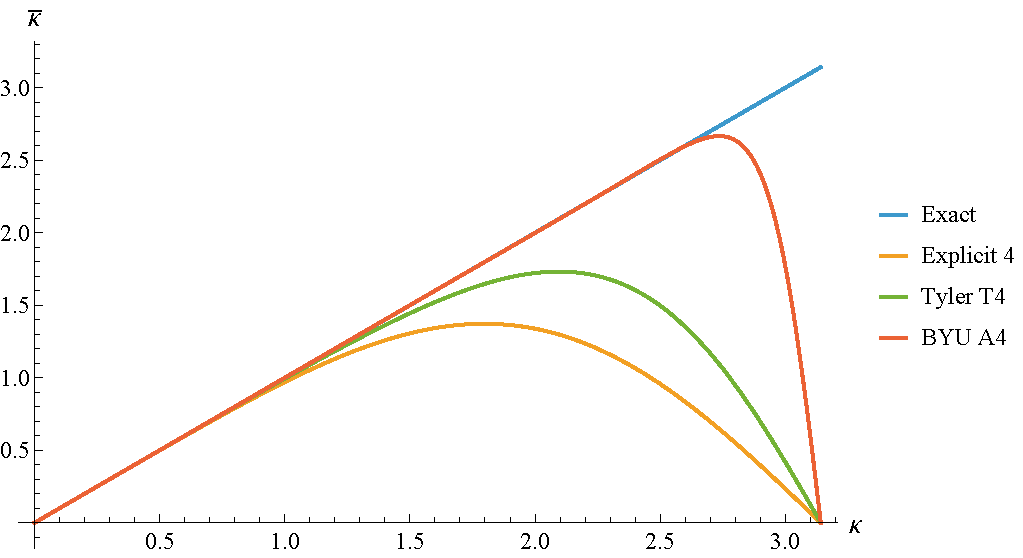
\includegraphics[width=\linewidth]{figures/1st_4th_Order_Spectral_Functions.pdf}
  \vspace{-.75cm}
  \caption{
   Comparison of spectral functions for several 4th order schemes: the explicit 4th order finite difference, a tridiagonal 4th order compact finite difference [ref Tyler], and a spectrally-optimized pentadiagonal 4th order compact finite difference [this work].
}
  \label{fig:4th_spectral_functions}
\end{figure}

We construct the following error quantity from the spectral function~\cite{yo}, namely 
\begin{equation}
E(\alpha_i, a_i) = \int_{0}^{r \pi}{\bigl[ \bar{\kappa} - \kappa \bigr]^2 D(\kappa)^2 \, d\kappa}
\end{equation}
where $D(\kappa)$ is simply the denominator in the spectral function, Eq. (\ref{spectral_function}). In general, an arbitrary weighting function can be used, but this form is chosen so that the integral can be computed analytically [ref Zhou Zhang 2011]. The parameter $r \in (0,1]$ in the upper bound of the integral is referred to as the ``fractional cutoff wavenumber,'' and represents the maximum modified wavenumber $\kappa$ over which the spectral error is optimized. It has been suggested [ref Chen 2023] to have a lower cutoff wavenumber around $0.5$ or $0.75$ to avoid over-optimization on higher-wavenumber modes, while others [ref Kim 2007] have used higher cutoff wavenumbers such as $0.839$. In this work, we develop several families of CFD operators for several values of the cutoff wavenumber from $0.6$ to $0.85$.

We minimize the error $E$ by substituting the solutions of the Taylor constraint equations up to a given order of accuracy for our ``fixed parameters'' and by imposing constraints of the form
\begin{equation}
\frac{\partial E}{\partial a_i} = 0,
\end{equation} 
for our ``free parameters.'' As the error quantity is quadratic with respect to its arguments, the resulting constraint equations form a linear system with respect to these free parameters, and hence yield a unique solution for a spectrally-optimized CFD scheme.

\subsubsection{Boundary Scheme}
If we wish to maintain the banded-diagonal form of these CFD operators on the boundary, we must develop a boundary closure using shifted stencils. However, it has been shown [refs] that centered stencils provide greater benefits in terms of accuracy and stability. Following the approach of Wu et al. [ref Kim 2024], we use a polynomial to extrapolate our function to grid points which lie beyond the boundary of our numerical domain.

If we have interior coefficients $\alpha_1$ through $\alpha_m$ on the LHS and $a_1$ through $a_k$ on the RHS, then the order of the extrapolation polynomial must be at least $\ell = 3k+m+1$.  
%$$
%P_{order} = 3k + m + 1.
%$$
We increase the order of this polynomial by one in order to introduce an extra free parameter in order to optimize the spectral behavior at and near the boundary. Following [ref Kim 2024], we construct the extrapolation polynomial, 
\begin{equation}
P(\hat{x}) = \sum_{s=0}^{\ell} p_s {\hat x}^s, 
\end{equation}
where ${\hat x} \equiv (x_j - x_0)/h$ and we use the information from the function and its derivatives: 
$$
\begin{cases}
    P(j) = f_j, \quad j = 0, 1, \dots, 2k\\
    \frac{dP}{dx}(j) = f'_j, \quad j = 0, 1, \dots, k + m\\
    \frac{d^n P}{dx^n}(\hat{y}) = 0.
\end{cases}
$$
The parameter $\hat{y}$ is a value which will be used for optimizing the boundary closures later on. The quantity $n$ is an arbitrary integer which should be at least greater than or equal to the order of accuracy of the scheme and at most less than or equal to the order of the extrapolation polynomial. We have found that a lower value of $n$ leads to a larger family of minima in our boundary error quantity and thus a larger family of error-optimized boundary closures.

Once we have solved the system above to find the coefficients of the extrapolation polynomial, we construct a centered stencil for each of the boundary nodes, substituting in the extrapolation polynomial at each of the grid points which lie beyond the domain. Finally, we can rearrange the resulting equations into the shifted stencils which can be implemented, and the shifted stencil boundary coefficients can be read off in terms of the free parameter $\hat{y}$ only.

As with the approach to optimizing the interior scheme, we Fourier transform the shifted boundary stencils to define a spectral function. For the $m$th boundary node, we find:
\begin{align*}
\bar{\kappa}_m(\kappa) &= \frac{1}{A_m(\kappa)^2 + B_m(\kappa)^2} \big[ A_m(\kappa) D_m(\kappa) - B_m(\kappa) C_m(\kappa)\\
&  \qquad\qquad\qquad - i (A_m(\kappa) C_m(\kappa) + B_m(\kappa) D_m(\kappa)) \big],
\end{align*}
where:
\begin{align*}
    A_m(\kappa) &= \sum_{j=0}^{3}{\gamma_{mj} \cos{(j \kappa)}}, \quad B_m(\kappa) = \sum_{j=0}^{3}{\gamma_{mj} \sin{(j \kappa)}},\\
    C_m(\kappa) &= \sum_{j=0}^{6}{a_{mj} \cos{(j \kappa)}}, \quad D_m(\kappa) = \sum_{j=0}^{6}{a_{mj} \sin{(j \kappa)}}.
\end{align*}
%\nate{TODO: Need to generalize the upper bounds of the sums, and also explain what $a_{mj}$ and $\gamma_{mj}$ are (the bd coefficients). In general I think I need to be a bit more clear in this section about the indices being used, maybe define some things like $n_L$ and $n_R$ at the beginning.}

Note that because the boundary stencils are shifted, their spectral functions have real and imaginary components, corresponding to both dispersive and dissipative behavior in the numerical scheme.

At this point, many different error quantities could be constructed in order to optimize specific features of the boundary closure. For example, an error quantity could be chosen to optimize only on the imaginary part of the spectral function in order to minimize unwanted dissipative modes. In the present work, we use the error quantity
$$
E_m = \int_{0}^{r \pi}{\Big[ \big| \Re(N_m(\kappa)) + i \Im(N_m(\kappa)) \big| - \kappa D_m(\kappa) \Big]^2 \ d\kappa}
$$
where $N_m(\kappa)$ and $D_m(\kappa)$ represent the numerator and denominator of the spectral function $\bar{\kappa}_m(\kappa)$, respectively; i.e., we have set:
\begin{align*}
    \Re(N_m(\kappa)) &= A(\kappa) D(\kappa) - B(\kappa) C(\kappa),\\
    \Im(N_m(\kappa)) &= -A(\kappa) C(\kappa) - B(\kappa) D(\kappa),\\
    D_m(\kappa) &= A(\kappa)^2 + B(\kappa)^2.
\end{align*}
Note that each boundary node has a spectral function and thus error quantity which is independent from each other. As each of the boundary coefficients $a_{mj}$ and $\gamma_{mj}$ only depend on the free parameter $\hat{y}$, then each error quantity also only depends on $\hat{y}$. Since the error functions are decoupled, we opt to use a separate free parameter $\hat{y}_m$ for each boundary node. Clearly, even with a similar weighting function to the interior scheme, this error integral is not analytically integrable, so we must numerically integrate the error quantity over a grid of possible values for $\hat{y}_m$. [ref Kim 2024] suggests testing $\hat{y}_m \in (-6,6)$, but we have found that the minima in the error are typically found for $\hat{y}_m \in (-1,5)$.

Since each boundary error function $E_m(\hat{y}_m)$ has several minima, we obtain a family of spectrally-optimized boundary closures by taking all possible combinations of optimal $\hat{y}_m$ values.

%\nate{Do we need a section talking about stability?}



%\subsection{Fourth-order operators}



% \subsection{EM4 Convergence}
% \begin{table}[p]
% \centering
% \small
% \setlength{\tabcolsep}{3.5pt}
% \renewcommand{\arraystretch}{1.15}
% \resizebox{\textwidth}{!}{%
% \begin{tabular}{lccccccc}
% \toprule
% Variable & A4\_3 & A6\_2 & C4\_1 & C6\_4 & E4 & E6 & E8 \\
% \textbf{Avg over vars} & \textbf{5.158} (6) & \textbf{6.618} (6) & \textbf{4.436} (6) & \textbf{5.788} (6) & \textbf{3.916} (6) & \textbf{5.799} (6) & \textbf{6.883} (6) \\
% \midrule
% U\_B0 & 5.088 $\pm$ 0.364 (7) & 6.473 $\pm$ 0.272 (7) & 4.460 $\pm$ 0.178 (7) & 6.075 $\pm$ 0.280 (7) & 3.918 $\pm$ 0.028 (7) & 5.783 $\pm$ 0.073 (7) & 6.574 $\pm$ 0.098 (7) \\
% U\_B1 & 5.079 $\pm$ 0.391 (7) & 6.472 $\pm$ 0.281 (7) & 4.367 $\pm$ 0.176 (7) & 6.228 $\pm$ 0.225 (7) & 3.918 $\pm$ 0.028 (7) & 5.783 $\pm$ 0.073 (7) & 6.574 $\pm$ 0.098 (7) \\
% U\_B2 & 5.166 $\pm$ 0.674 (7) & 6.639 $\pm$ 0.314 (7) & 4.241 $\pm$ 0.194 (7) & 6.613 $\pm$ 0.286 (7) & 3.899 $\pm$ 0.058 (7) & 5.779 $\pm$ 0.115 (7) & 6.743 $\pm$ 0.104 (7) \\
% U\_E0 & 5.390 $\pm$ 0.344 (7) & 6.693 $\pm$ 0.470 (7) & 4.259 $\pm$ 0.123 (7) & 6.548 $\pm$ 0.232 (7) & 3.908 $\pm$ 0.038 (7) & 5.790 $\pm$ 0.084 (7) & 6.822 $\pm$ 0.196 (7) \\
% U\_E1 & 5.373 $\pm$ 0.346 (7) & 6.679 $\pm$ 0.450 (7) & 4.269 $\pm$ 0.122 (7) & 6.512 $\pm$ 0.257 (7) & 3.908 $\pm$ 0.038 (7) & 5.790 $\pm$ 0.084 (7) & 6.822 $\pm$ 0.196 (7) \\
% U\_E2 & 4.853 $\pm$ 0.284 (7) & 6.751 $\pm$ 0.292 (7) & 5.018 $\pm$ 0.165 (7) & 2.754 $\pm$ 0.894 (7) & 3.946 $\pm$ 0.012 (7) & 5.869 $\pm$ 0.017 (7) & 7.767 $\pm$ 0.028 (7) \\
% \bottomrule
% \end{tabular}%
% }
% \caption{A\_05: Evolved variables (cells show mean ± std (N); avg row shows weighted mean over variables, with (\#vars))}
% \end{table}
% \begin{figure}\centering
%   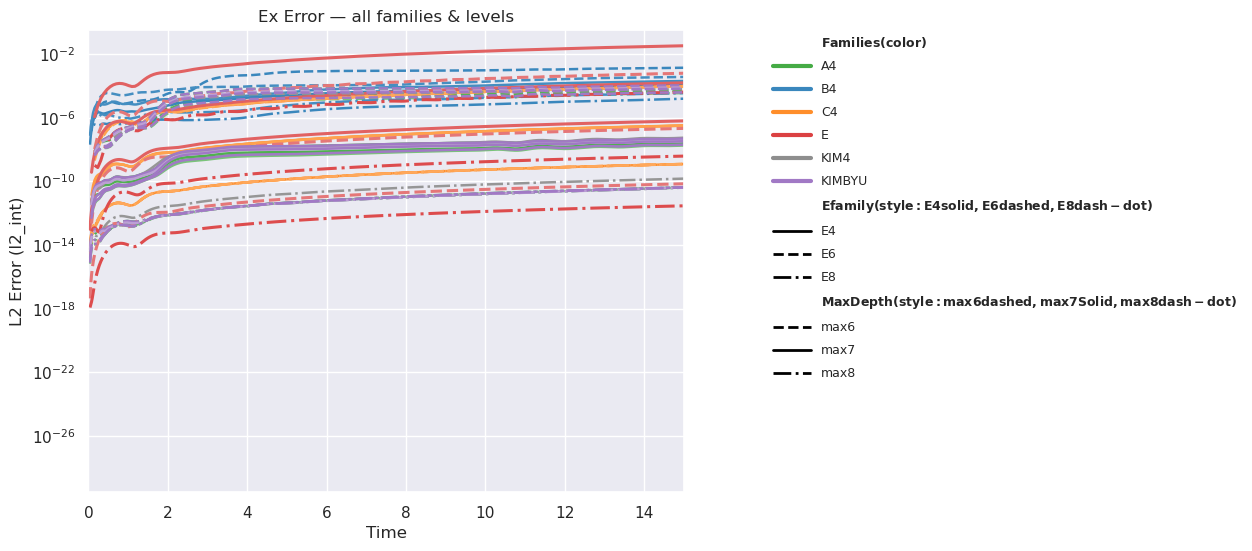
\includegraphics[width=\linewidth]{figures/U_E0_DIFF__ALL_FAMILIES.png}  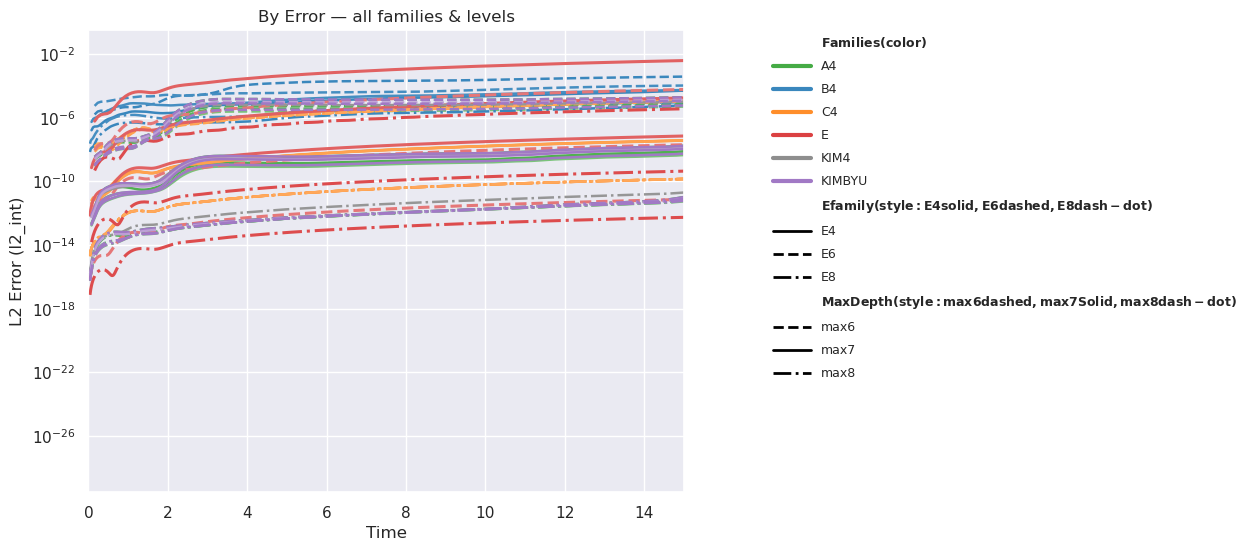
\includegraphics[width=\linewidth]{figures/U_B1_DIFF__ALL_FAMILIES.png}
%   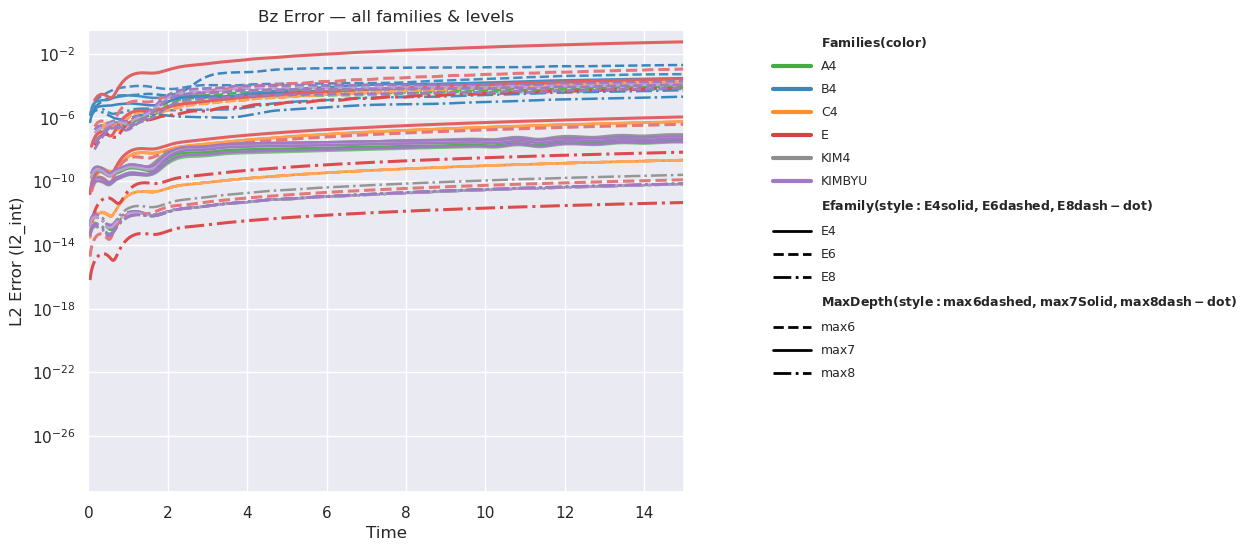
\includegraphics[width=\linewidth]{figures/U_B2_DIFF__ALL_FAMILIES.png}
%   \vspace{-.75cm}
%   \caption{
%     Comparison of error in the magnetic field component, $B_y$, for different CFD and explicit schemes.   component  for $q=4$. 
%     % describe sub-plots
%     We see .  blah blah blah
%   }
%   \label{fig:B_y_allfams}
% \end{figure}


\section*{Symbolic Matrices}
This is specifically the formulation of the 1A family of matrices.

\[
\mathbf{P} = 
\left(
\begin{array}{ccccccccccc}
1 & \gamma_{01} & \gamma_{02} & 0 & 0 & 0 & 0 & 0 & \cdots & 0 \\
\gamma_{10} & 1 & \gamma_{12} & \gamma_{13} & 0 & 0 & 0 & 0 & \cdots & 0 \\
\gamma_{20} & \gamma_{21} & 1 & \gamma_{23} & \gamma_{24} & 0 & 0 & 0 & \cdots & 0 \\
0 & \beta & \alpha & 1 & \alpha & \beta & 0 & 0 & \cdots & 0 \\
\vdots & \ddots & \ddots & \ddots & \ddots & \ddots & \ddots & \ddots & \ddots & \vdots \\
0 & \cdots & 0 & 0 & \beta & \alpha & 1 & \alpha & \beta & 0 \\
0 & \cdots & 0 & 0 & 0 & \gamma_{24} & \gamma_{23} & 1 & \gamma_{12} & 0 \\
0 & \cdots & 0 & 0 & 0 & 0 & \gamma_{13} & \gamma_{12} & 1 & \gamma_{10} \\
0 & \cdots & 0 & 0 & 0 & 0 & 0 & \gamma_{02} & \gamma_{01} & 1 \\
\end{array}
\right)
\]

\[
\mathbf{Q} = 
\left(
\begin{array}{ccccccccccc}
a_{00} & a_{01} & a_{02} & a_{03} & a_{04} & a_{05} & a_{06} & 0 & \cdots & 0 \\
a_{10} & a_{11} & a_{12} & a_{13} & a_{14} & a_{15} & a_{16} & 0 & \cdots & 0 \\
a_{20} & a_{21} & a_{22} & a_{23} & a_{24} & a_{25} & a_{26} & 0 & \cdots & 0 \\
-a_3 & -a_2 & -a_1 & 0 & a_1 & a_2 & a_3 & 0 & \cdots & 0 \\
\vdots & \ddots & \ddots & \ddots & \ddots & \ddots & \ddots & \ddots & \ddots & \vdots \\
0 & \cdots & 0 & -a_3 & -a_2 & -a_1 & 0 & a_1 & a_2 & a_3 \\
0 & \cdots & 0 & -a_{26} & -a_{25} & -a_{24} & -a_{23} & -a_{22} & -a_{21} & -a_{20} \\
0 & \cdots & 0 & -a_{16} & -a_{15} & -a_{14} & -a_{13} & -a_{12} & -a_{11} & -a_{10} \\
0 & \cdots & 0 & -a_{06} & -a_{05} & -a_{04} & -a_{03} & -a_{02} & -a_{01} & -a_{00} \\
\end{array}
\right)
\]


% \section*{Tables of Coefficients}
% The specific coefficients in this table are for 1A4 Op 5.

% - How do I get the spacing to line up when there's negative signs? And also with the ``blank'' entries? I was trying to somewhat mimic the format of Kim 2024's coefficient tables.

% - It may be better to put the interior coefficients separately if we are listing coefficients for several A4 operators; they have the same interior but different boundary coefficients (for example, A4 Op 2 vs. A4 Op 13).

% - Is it worth noting the condition that $a_{ii} = -\sum_{k \neq i}{a_{ik}}$? Kim often omits the $a_{ii}$ entries from his coefficient tables because of this, I personally find it helpful and cleaner to have it filled in, but we have verified before that the coefficients we're getting satisfy this condition, as they should.

% \begin{table}[h!]
% \centering
% \begin{tabular}{|c|c c c|} 
%  \hline
%  Interior Nodes & Node 0 & Node 1 & Node 2 \\
%  \hline
%  $\alpha$ \quad $0.577046020129014$ & - \quad - & $\gamma_{10}$ \quad $0.081850642218291$ & $\gamma_{20}$ \quad $0.010832502509738$ \\
%  $\beta$ \quad $0.089008368450770$ & $\gamma_{01}$ \quad $9.820500862970050$ & - \quad - & $\gamma_{21}$ \quad $0.238186806866178$ \\
%  - \quad - & $\gamma_{02}$ \quad $10.282867809058310$ & $\gamma_{12}$ \quad $1.689062748171480$ & - \quad - \\
%  - \quad - & - \quad - & $\gamma_{13}$ \quad $0.496147893138870$ & $\gamma_{23}$ \quad $1.128279076992181$ \\
%  - \quad - & - \quad - & - \quad - & $\gamma_{24}$ \quad $0.288649699198454$ \\
%  \hline
%  $a_1$ \quad $0.651707844090089$ & $a_{00}$ \quad $-3.734452513805820$ & $a_{10}$ \quad $-0.318509096234275$ & $a_{20}$ \quad $-0.046786865516800$ \\
%  $a_2$ \quad $0.248158826270106$ & $a_{01}$ \quad $-10.765902315893960$ & $a_{11}$ \quad $-1.396944235854646$ & $a_{21}$ \quad $-0.510448282160808$ \\
%  $a_3$ \quad $0.006009630649828$ & $a_{02}$ \quad $11.158777481815810$ & $a_{12}$ \quad $0.536401605870469$ & $a_{22}$ \quad $-0.770033072247311$ \\
%  - \quad - & $a_{03}$ \quad $3.893279579988119$ & $a_{13}$ \quad $1.122316892895001$ & $a_{23}$ \quad $0.622893361976584$ \\
%  - \quad - & $a_{04}$ \quad $-0.638983973815703$ & $a_{14}$ \quad $0.059450604503400$ & $a_{24}$ \quad $0.672712515935698$ \\
%  - \quad - & $a_{05}$ \quad $0.095877273974209$ & $a_{15}$ \quad $-0.002743838025071$ & $a_{25}$ \quad $0.033041689527406$ \\
%  - \quad - & $a_{06}$ \quad $-0.008595531676509$ & $a_{16}$ \quad $0.000028066844770$ & $a_{26}$ \quad $-0.001379347514431$ \\
%  \hline
% \end{tabular}
% \caption{Coefficients for First Derivative A4 Operator \#5}
% \label{table:1stA4Op5coeff}
% \end{table}


%\subsection{Sixth-order operators}

\section{Test cases}

Having sketched the process of computing boundary-closed CFD operators for a given order of accuracy, we here present several tests of these operators as applied in specific systems of PDEs.  

We begin with a 1D nonlinear system, namely Burgers' equation.  We also consider Maxwell's equations in full 3D together with hyperbolic divergence cleaning.  We return to nonlinear problems with a 3D nonlinear sigma model and conclude with the Einstein equations with the evolution of Teukolsky gravitational waves. 

In each case, the basic results are similar.  Namely, the use of CFDs at some accuracy order perform better than a comparable explicit FD scheme, sometimes by more than an order of magnitude as measured by.  Effectively, the CFDs are providing comparable error profiles at half the resolution of the FDs.  


%\subsection{Classical wave equation}



\subsection{One-Dimensional Nonlinear Burgers'}

Our first test uses the nonlinear one-dimensional viscous Burgers' Equation,
\begin{equation}
\label{eq:BurgersEq}
\frac{\partial f}{\partial t}
=
-f\frac{\partial f}{\partial x}
+
\frac{\partial^2 f}{\partial x^2},
\qquad
-\infty < x < \infty,
\qquad
t \ge 0.
\end{equation}
where the solution $f(x,t)$ depends only on $x$ and $t$, and the viscosity coefficient is fixed at $1$ for simplicity.

This admits a closed form solution against which we will compare the numerical solution.  It is 
\begin{equation}
    f(x,t) = \frac{2}{1+e^{x-t}}.
\end{equation}
The initial condition, of course, is thus 
\begin{equation}
    \phi(x,t=0) = \frac{2}{1+e^x}.
\end{equation}
%This initial condition is chosen because it admits a closed-form analytical solution for comparison. The corresponding solution is

In solving this problem numerically, we approximate both first and second spatial derivatives using CFDs and explicit FDs separately.  The time integration is done using a fourth order Runge-Kutta scheme as will be true for all subsequent tests as well.   
%our tests.  This will leave the equation in a semidiscretized form, from which we may advance the solutions in time using a method-of-lines approach with a stable time-integration method.

To focus in this test problem on the interior parts of the CFDs, we take a domain of $-100 \le x \le 100$ and limit the simulation time to $0 \le t < 50$. Because the solution approaches constant states far from the transition region near $x=t$, fixed Dirichlet boundary conditions provide an accurate approximation on the truncated domain.  Appropriate boundary-closed operators continue to be use

The continuous domain $[-100,100]$ is divided into $N$ uniform cells of width $h$. Using a grid defined at the cell boundaries, we will have $N+1$ grid points to represent the domain. Defining $\phi_i(t) = \phi(-100 + ih,t)$ to be the $i$th point of the solution along the domain, with $i$ ranging from $0$ to $N$, we can write equation \ref{eq:BurgersEq} in the semidiscrete form:
\begin{equation}
    \frac{d \phi_i}{d t} = -\phi_i \textbf{D}_1 \phi_i + \textbf{D}_2\phi_i,
\end{equation}
where $\textbf{D}_1$ and $\textbf{D}_2$ denote the discrete first- and second-derivative operators, respectively

From here, the standard fourth-order Runge--Kutta (RK4) method is implemented to advance our solution in time. At each time step, including the intermediary stages in the integration, the Dirichlet boundary conditions are imposed on the first and last entries of the solution. This process is repeated for select resolutions of $N$, $2N$, and $4N$, and the $L_2$-norm of the error when compared with the analytic solution is calculated.

Figures \ref{fig:4th_burgers_error} and \ref{fig:6th_burgers_error} both show the analytic error of these evolutions using 4 different operators at three different resolutions. The values chosen are $N=200,400,800$ for the low, medium, and high resolutions respectively. The E4 and E6 operators are both standard explicit finite difference schemes with 4th- and 6th-order accuracy for both first and second derivatives. The A4 and C4 operators are two of the optimized compacts schemes at 4th order for the first derivative, with the choice of a non-optimized compact tridiagonal scheme for the second derivative. Likewise, the C6 operator is another optimized 6th order compact scheme for the first derivative in tandem with a non-optimized tridiagonal compact scheme in the second derivative. In both cases, the compact schemes at low resolutions perform almost as well or better than the explicit schemes at a resolution with twice as many points. This shows a definite improvement in accuracy with the compact schemes.

\begin{figure}\centering
  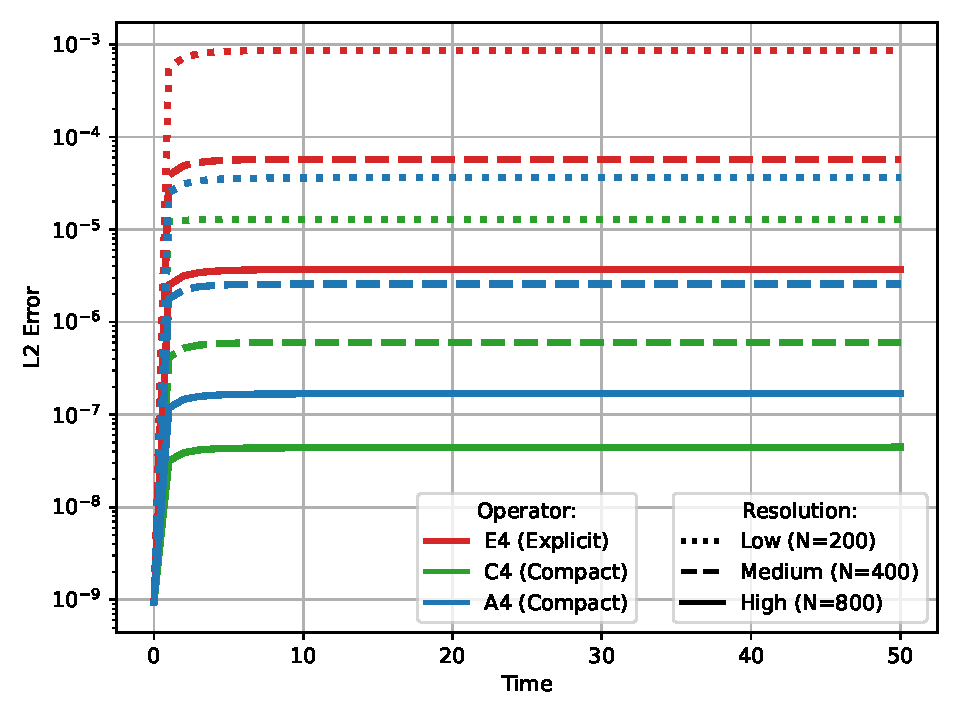
\includegraphics[width=\linewidth]{figures/4th_order_Burgers.pdf}
  %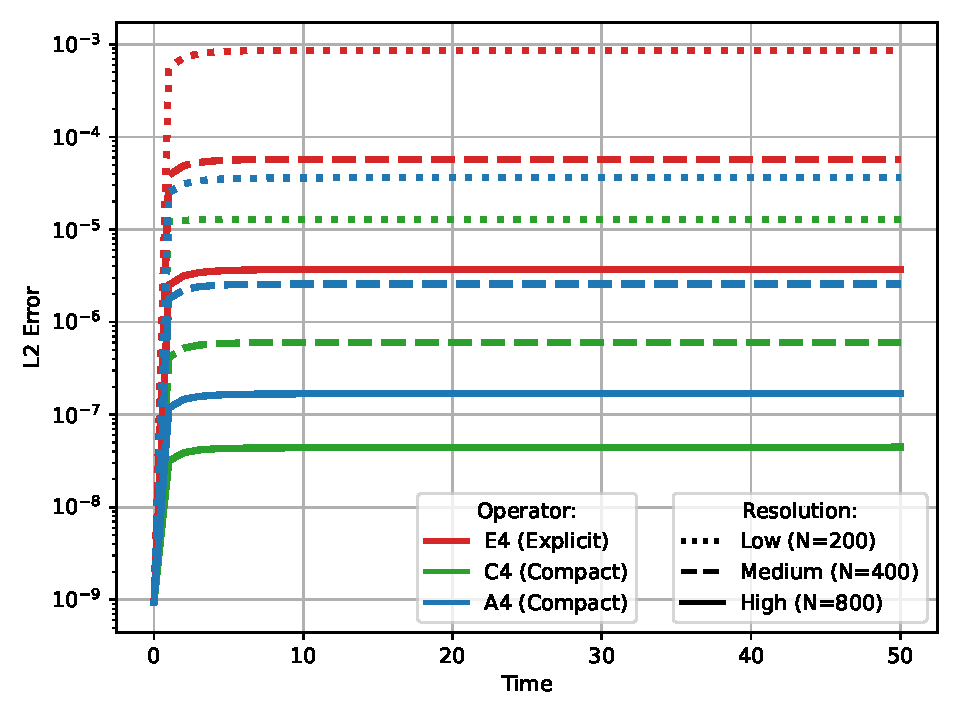
\includegraphics[width=\linewidth]{figures/4th_order_Burgers.pdf}
  \vspace{-.75cm}
  \caption{
   Analytic error of Burger's equation at different resolutions with 4th order operators
}
  \label{fig:4th_burgers_error}
\end{figure}

\begin{figure}\centering
  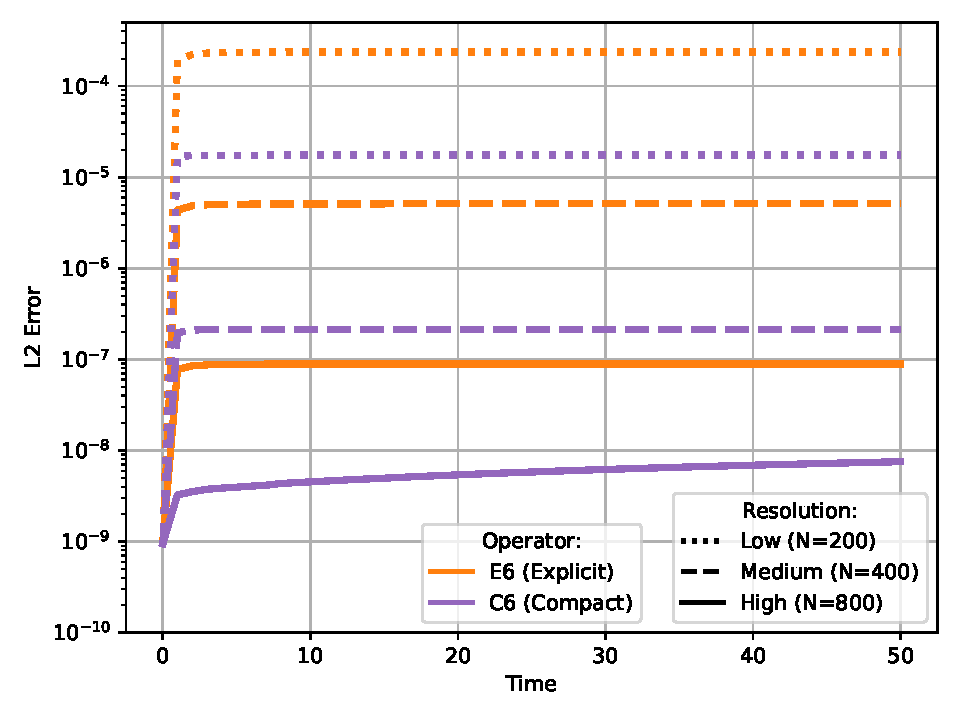
\includegraphics[width=\linewidth]{figures/6th_order_Burgers.pdf}
  %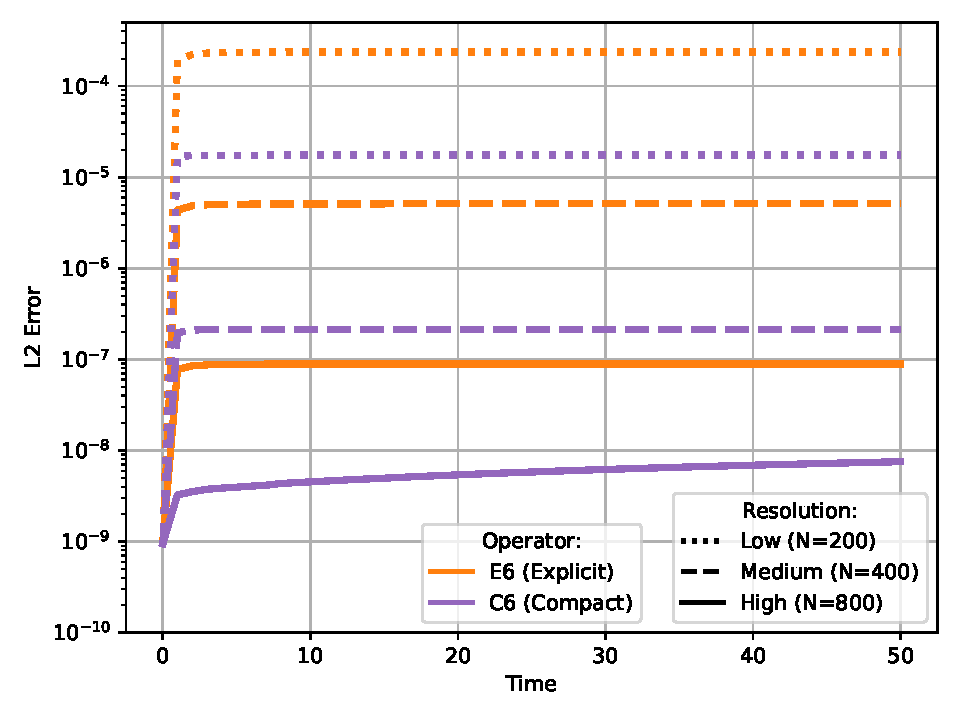
\includegraphics[width=\linewidth]{figures/6th_order_Burgers.pdf}
  \vspace{-.75cm}
  \caption{
   Analytic error of Burger's equation at different resolutions with 6th order operators
}
  \label{fig:6th_burgers_error}
\end{figure}


\subsection{Maxwell equations}
\label{sec:maxwell_equations}

The Maxwell equations provide a useful physical system for testing and
comparing different computational methods. They form a linear system with
known solutions, while retaining sufficient structure to make the numerical
tests nontrivial. For example, the Maxwell equations contain hyperbolic
evolution equations for the electric and magnetic fields, $\mathbf{E}$ and
$\mathbf{B}$, respectively,
\begin{equation}
\label{eq:maxwell_evolution}
\frac{\partial \mathbf{E}}{\partial t}
    = \nabla \times \mathbf{B},
\qquad
\frac{\partial \mathbf{B}}{\partial t}
    = -\nabla \times \mathbf{E},
\end{equation}
as well as constraint equations that must hold at all times,
\begin{equation}
\label{eq:maxwell_constraints}
\nabla \cdot \mathbf{E} = 0,
\qquad
\nabla \cdot \mathbf{B} = 0.
\end{equation}
Moreover, these equations can be written in different formulations that
mimic properties of more complicated systems. For example, Knapp
et al.~\cite{Knapp:2002fm} considered a formulation intended to reproduce
features encountered when solving the Einstein field equations in numerical
relativity.

In this work, we consider the standard Maxwell system with additional
constraint damping fields, $\Psi$ and $\Phi$, which are used to damp
violations of the electric and magnetic constraints:
\begin{align}
\partial_t E_i
    &= \epsilon_{ijk}\nabla^j B^k - 4\pi J_i - \partial_i \Psi,
\label{eq:maxwell_evolution_E}
\\
\partial_t B_i
    &= -\epsilon_{ijk}\nabla^j E^k + \partial_i \Phi,
\label{eq:maxwell_evolution_B}
\\
\partial_t \Psi
    &= 4\pi \rho_e - \partial_i E^i - \kappa_1 \Psi,
\label{eq:maxwell_evolution_Psi}
\\
\partial_t \Phi
    &= \partial_i B^i - \kappa_2 \Phi,
\label{eq:maxwell_evolution_Phi}
\\
0
    &= \nabla_i E^i - 4\pi \rho_e,
\label{eq:maxwell_constraint_E}
\\
0
    &= \nabla_i B^i.
\label{eq:maxwell_constraint_B}
\end{align}

% We also consider a formulation analogous to the BSSN formulation of general relativity:
%
% \begin{align}
% \partial_t E_i
%     &= -\nabla^j \nabla_j A_i + \nabla_i \Gamma - 4\pi J_i,
% \\
% \partial_t A_i
%     &= -E_i - \nabla_i \psi,
% \\
% \partial_t \Gamma
%     &= -4\pi \rho_e - \nabla_i \nabla^i \psi,
% \\
% \partial_t \psi
%     &= -\nabla_i A^i,
% \\
% 0
%     &= \nabla_i E^i - 4\pi \rho_e,
% \\
% 0
%     &= \nabla_i A^i - \Gamma.
% \end{align}
%
% This system also includes constraint damping, with $\Gamma$ allowing for
% the elimination of mixed derivatives.

As a test case, we use a dipolar solution of Maxwell's equations. In
particular, we choose initial data from the exact solution given by Knapp
et al.~\cite{Knapp:2002fm}:
\begin{equation}
\label{eq:maxwell_dipole_potential}
A^{\hat{\phi}}
=
\mathcal{A}\sin\theta
\left[
\frac{e^{-\lambda v^2}-e^{-\lambda u^2}}{r^2}
-
2\lambda
\frac{v e^{-\lambda v^2}+u e^{-\lambda u^2}}{r}
\right].
\end{equation}
The corresponding electric field is
\begin{equation}
\label{eq:maxwell_dipole_electric_field}
\begin{aligned}
E^{\hat{\phi}}
&=
2\lambda\mathcal{A}\sin\theta
\biggl[
\frac{
    v e^{-\lambda v^2}
    -
    u e^{-\lambda u^2}
}{r^2}
\\
&\qquad\qquad
+
\frac{1}{r}
\bigl[
    (1-2\lambda v^2)e^{-\lambda v^2}
    +
    (1-2\lambda u^2)e^{-\lambda u^2}
\bigr]
\biggr].
\end{aligned}
\end{equation}
Here
\begin{equation}
u = t-r,
\qquad
v = t+r,
\end{equation}
are the retarded and advanced time coordinates, respectively.
The parameter $\mathcal{A}$ sets the initial amplitude, while $\lambda$
controls the width of the pulse. The corresponding Cartesian components are
obtained using the standard coordinate transformation from spherical to
Cartesian coordinates.

The advantage of these initial data is that they admit an analytic solution.
In our experiments, we set $\mathcal{A}=1.0$ and $\lambda=0.5$. By comparing
the evolved solution against the analytic solution, we obtain a direct
measure of the error associated with each finite difference operator. A
representative evolution is shown in Fig.~\ref{fig:em4_e0_panel}.

\begin{figure}[t]
    \centering
    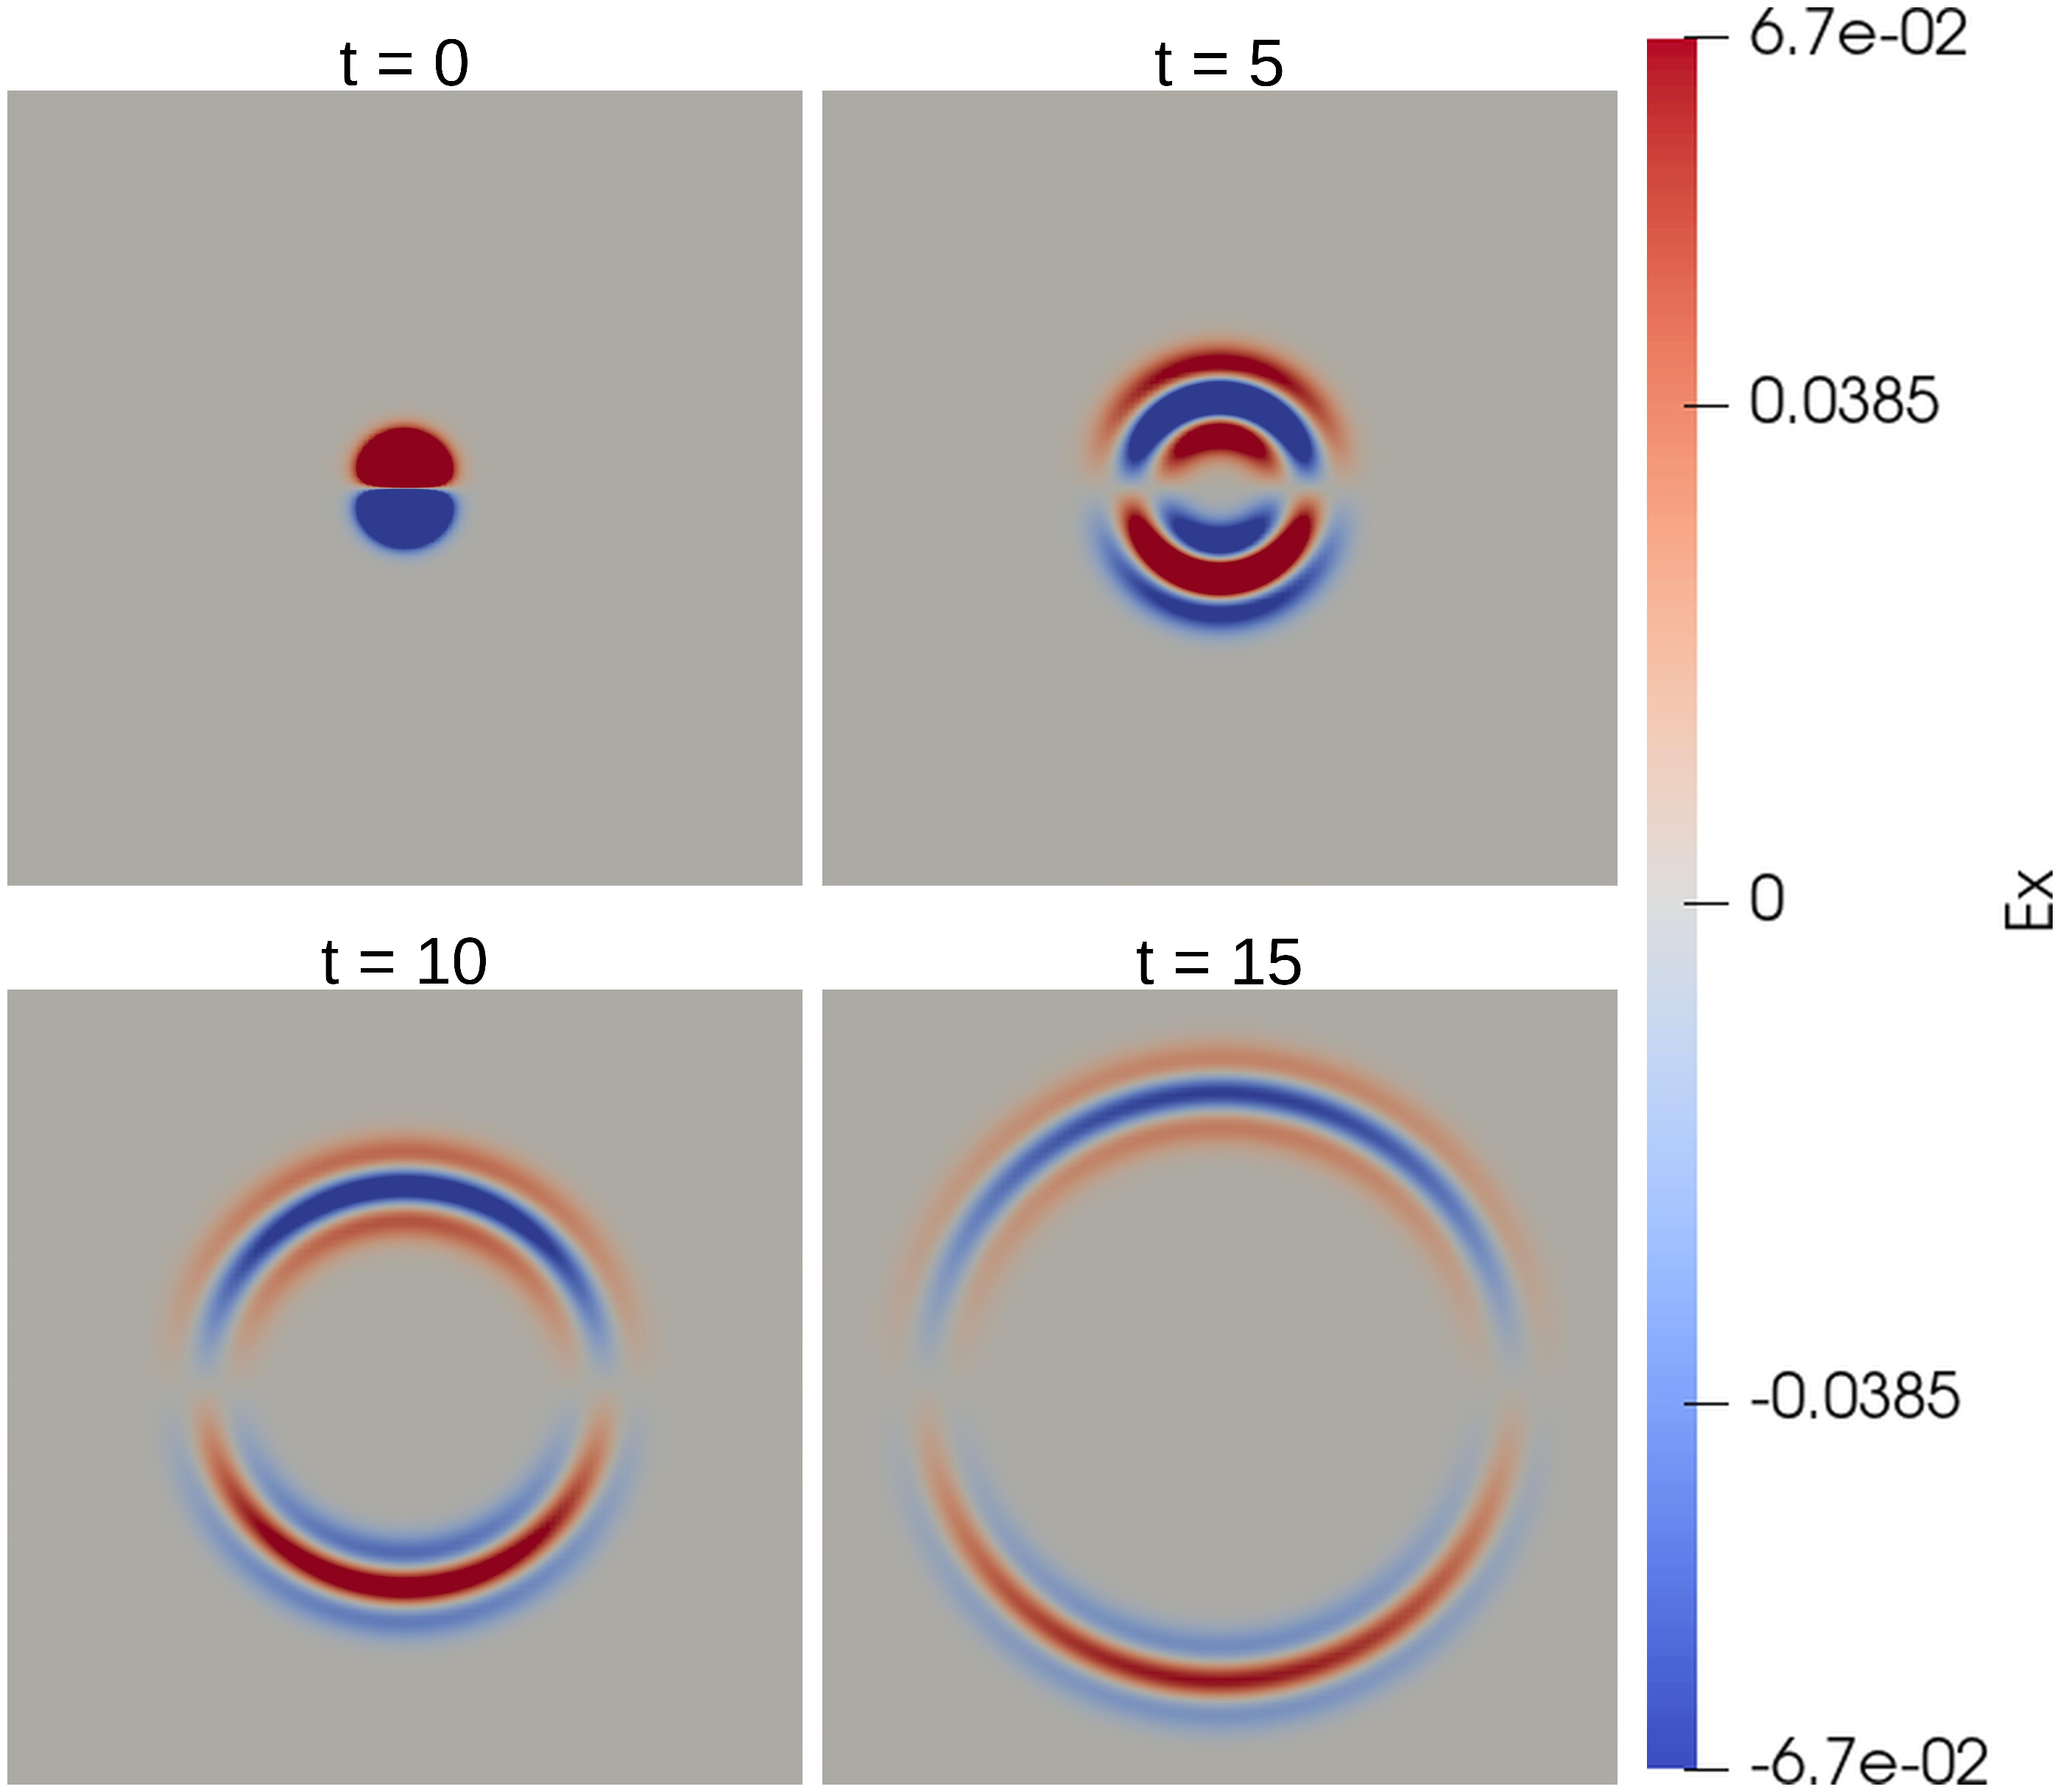
\includegraphics[width=\columnwidth]{figures/E0_panel.pdf}
    \caption{
    Evolution of the electric field component $E_x$ for the dipolar Maxwell
    test problem. The panels show representative snapshots during the
    evolution, with a shared color scale shown on the right. The initial
    dipolar pulse gradually propagates outward.
    }
    \label{fig:em4_e0_panel}
\end{figure}

\paragraph{Fourth Order Operators}

\begin{figure}[t]
    \centering
    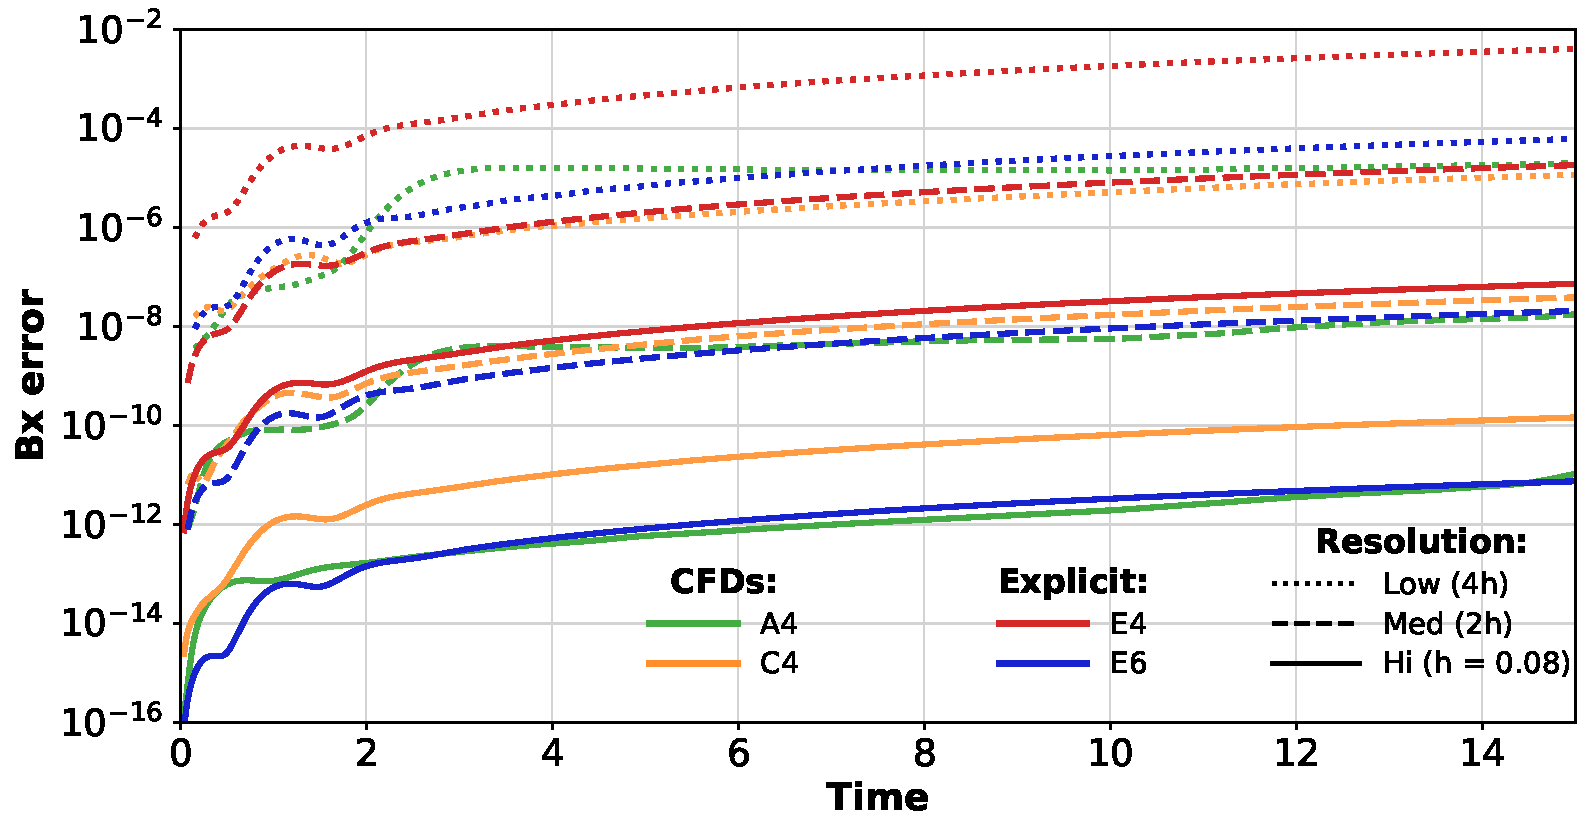
\includegraphics[width=\linewidth]{figures/U_B0_DIFF__ALL_FAMILIES.pdf}
    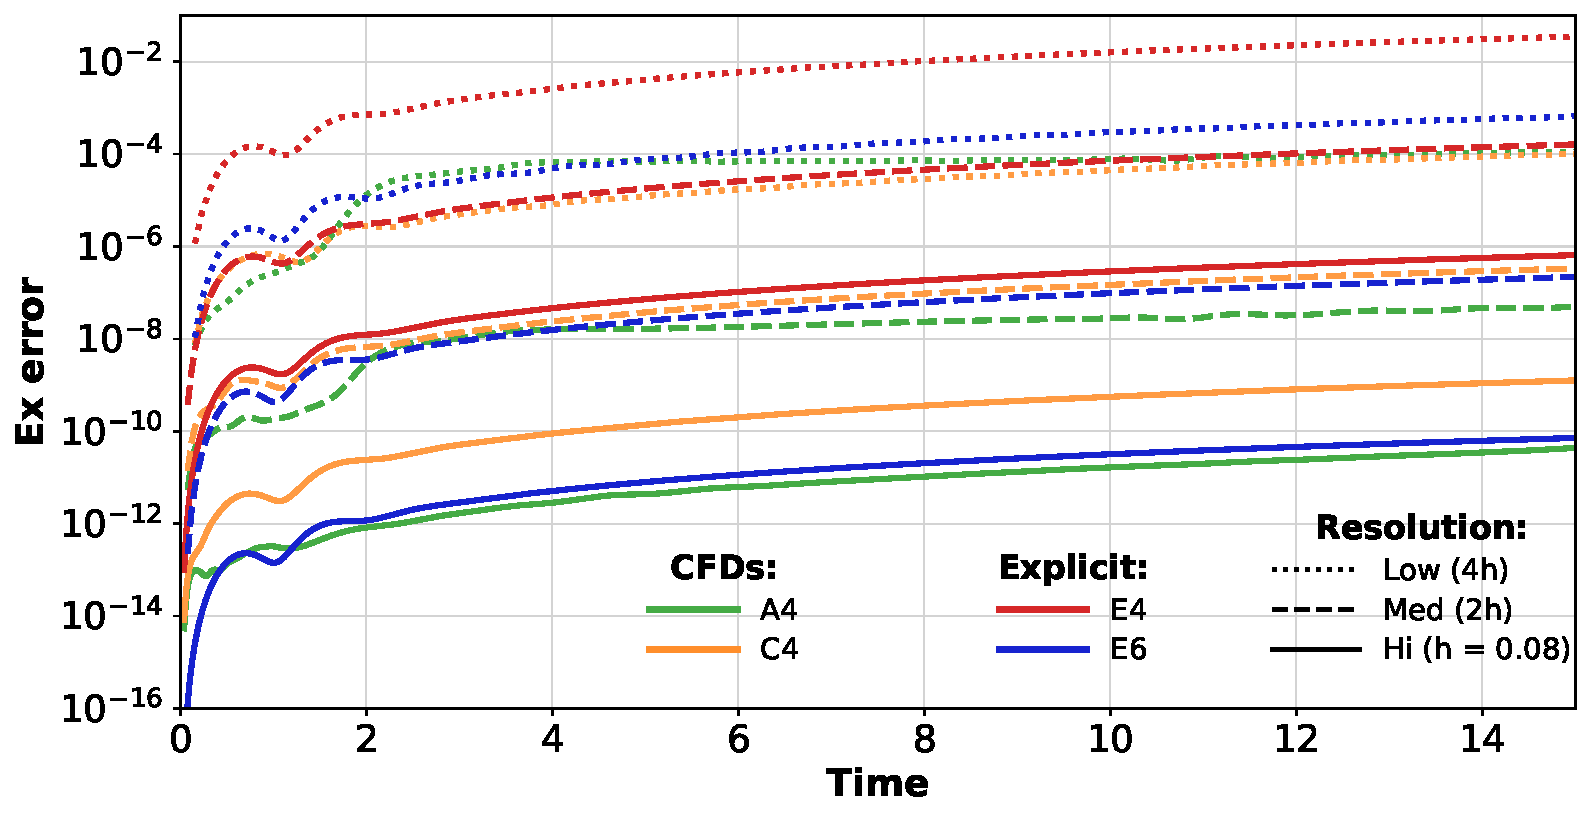
\includegraphics[width=\linewidth]{figures/U_E0_DIFF__ALL_FAMILIES.pdf}
    %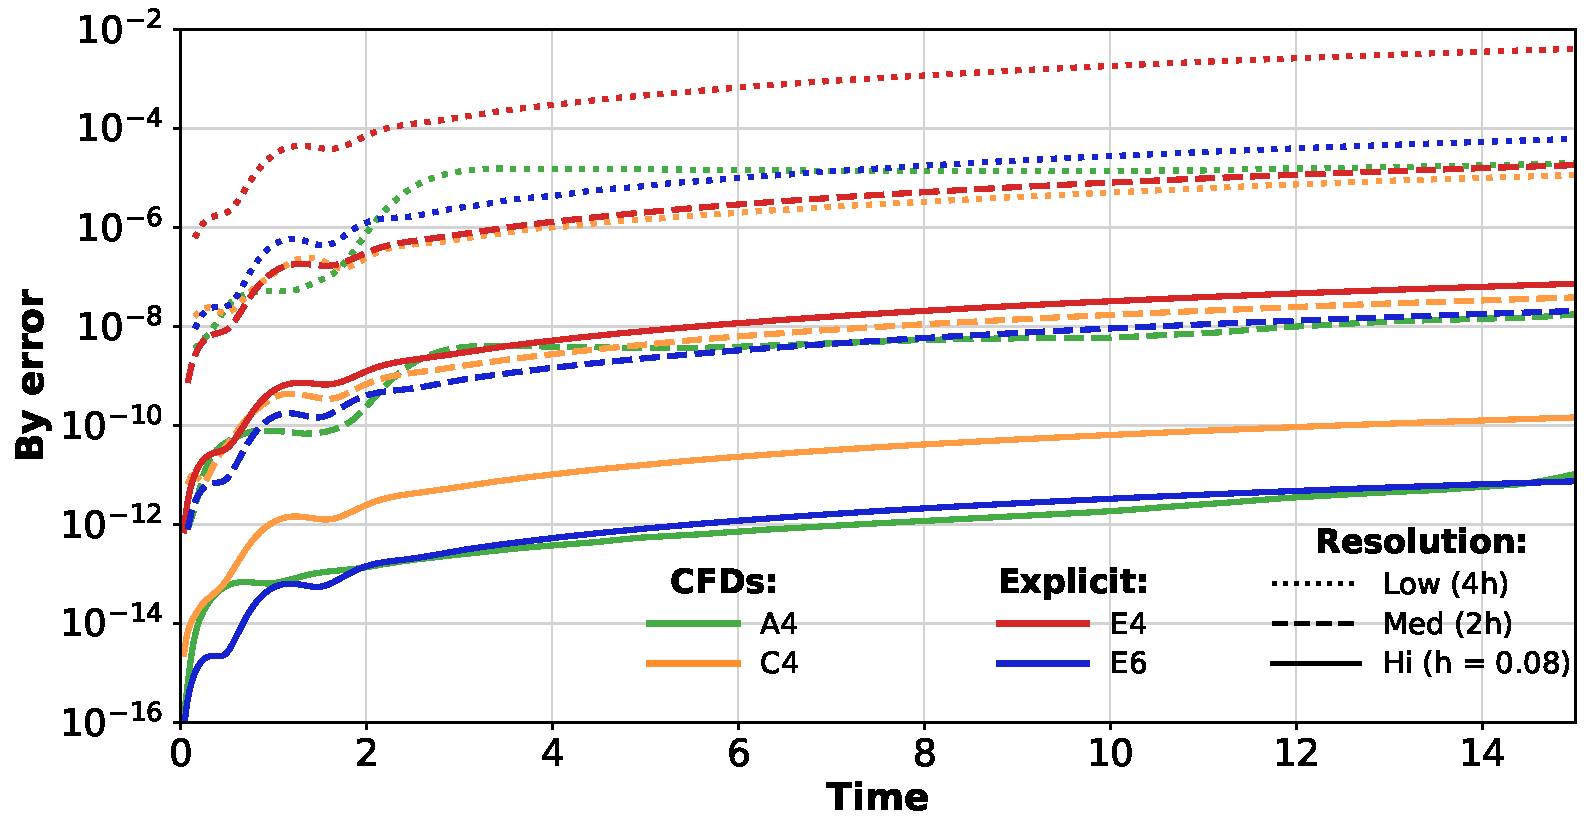
\includegraphics[width=\linewidth]{figures/U_B1_DIFF__ALL_FAMILIES.pdf}
    %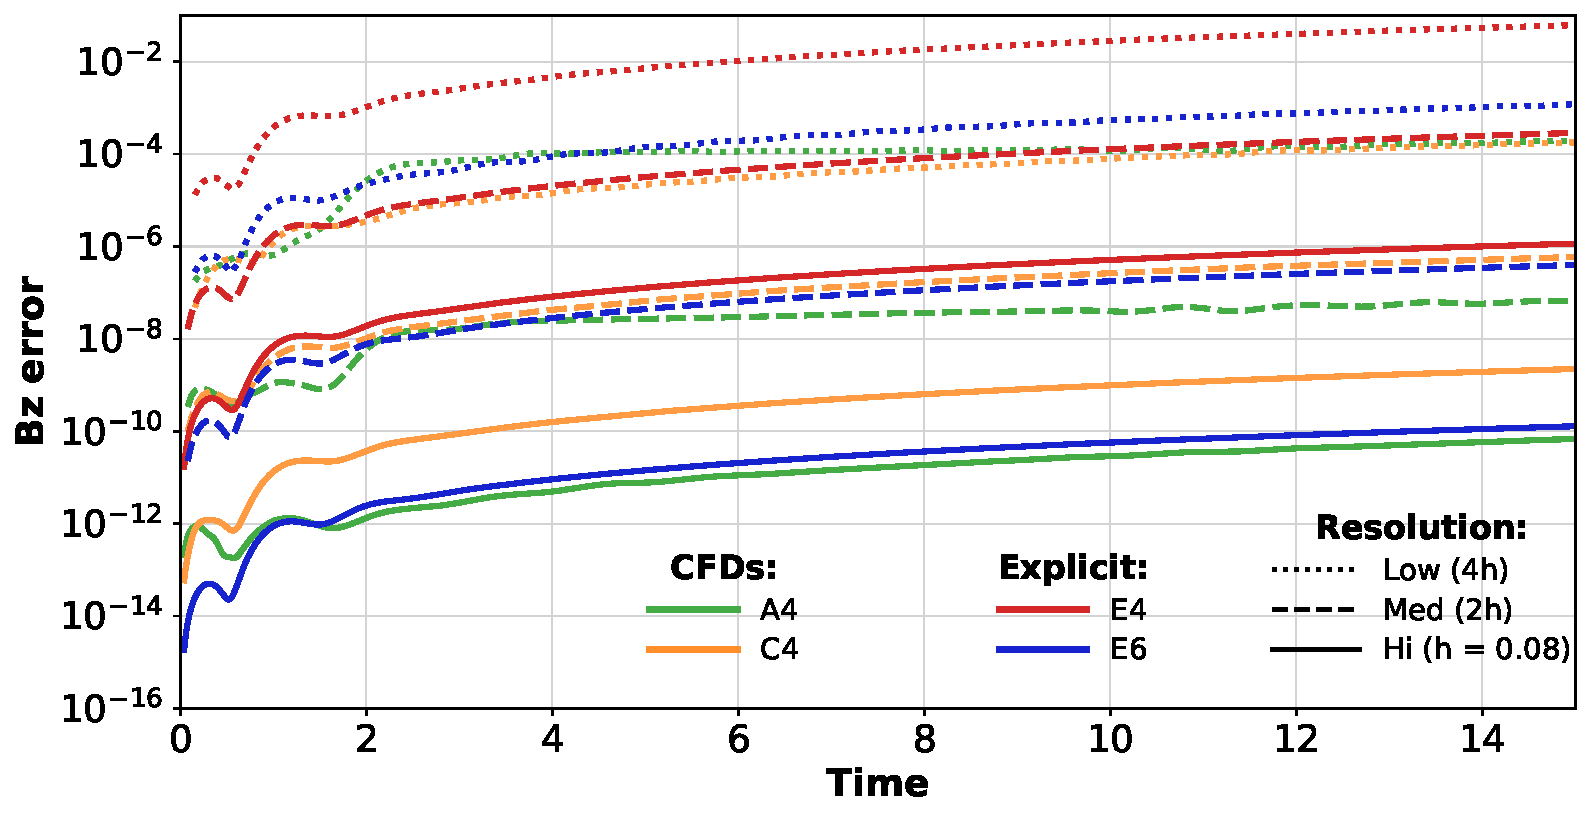
\includegraphics[width=\linewidth]{figures/U_B2_DIFF__ALL_FAMILIES.pdf}
    %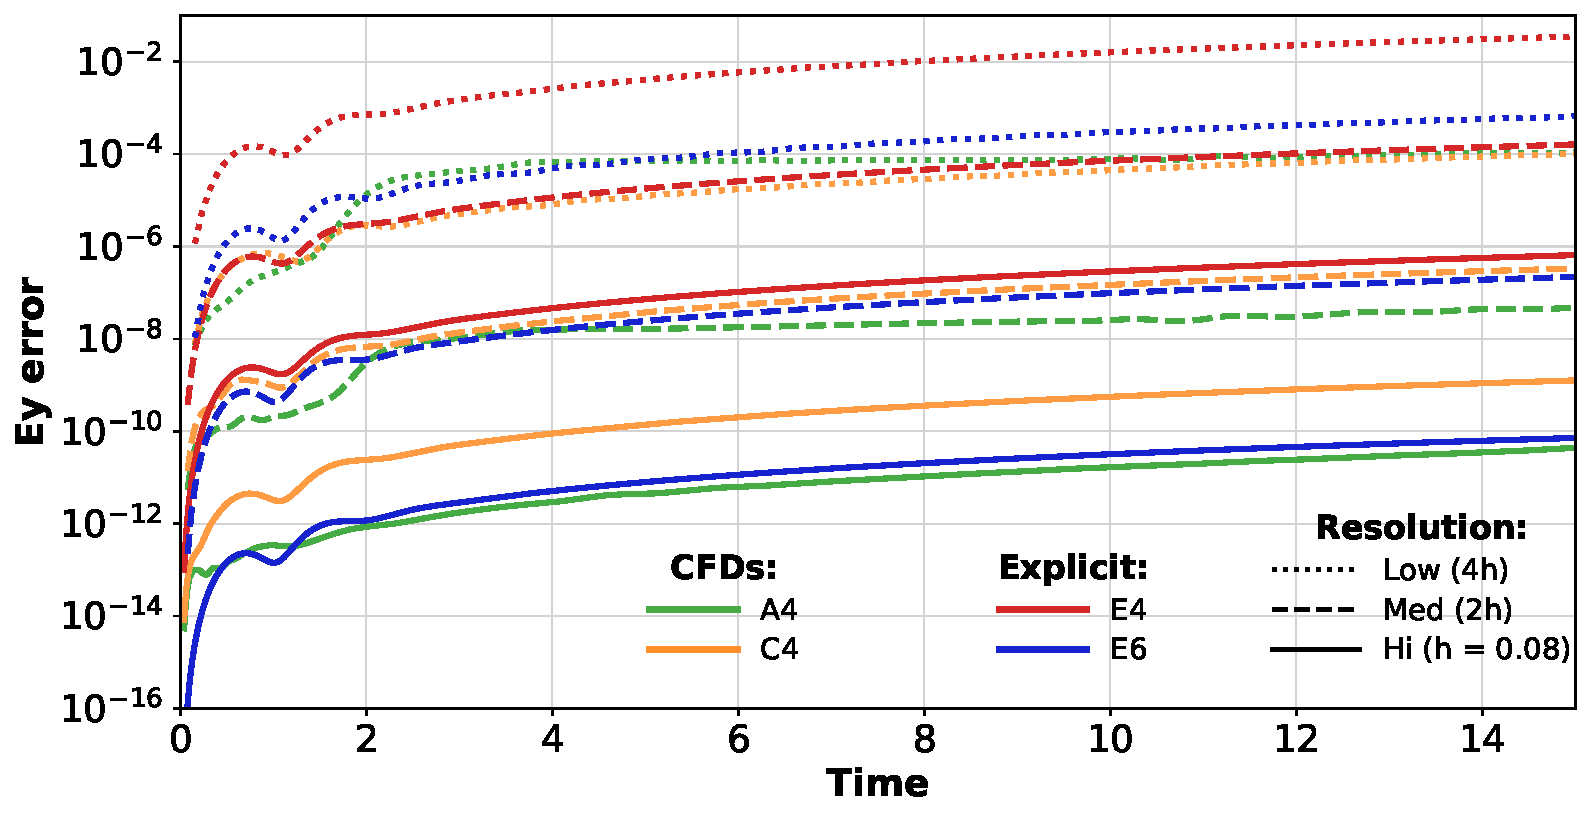
\includegraphics[width=\linewidth]{figures/U_E1_DIFF__ALL_FAMILIES.pdf}
    %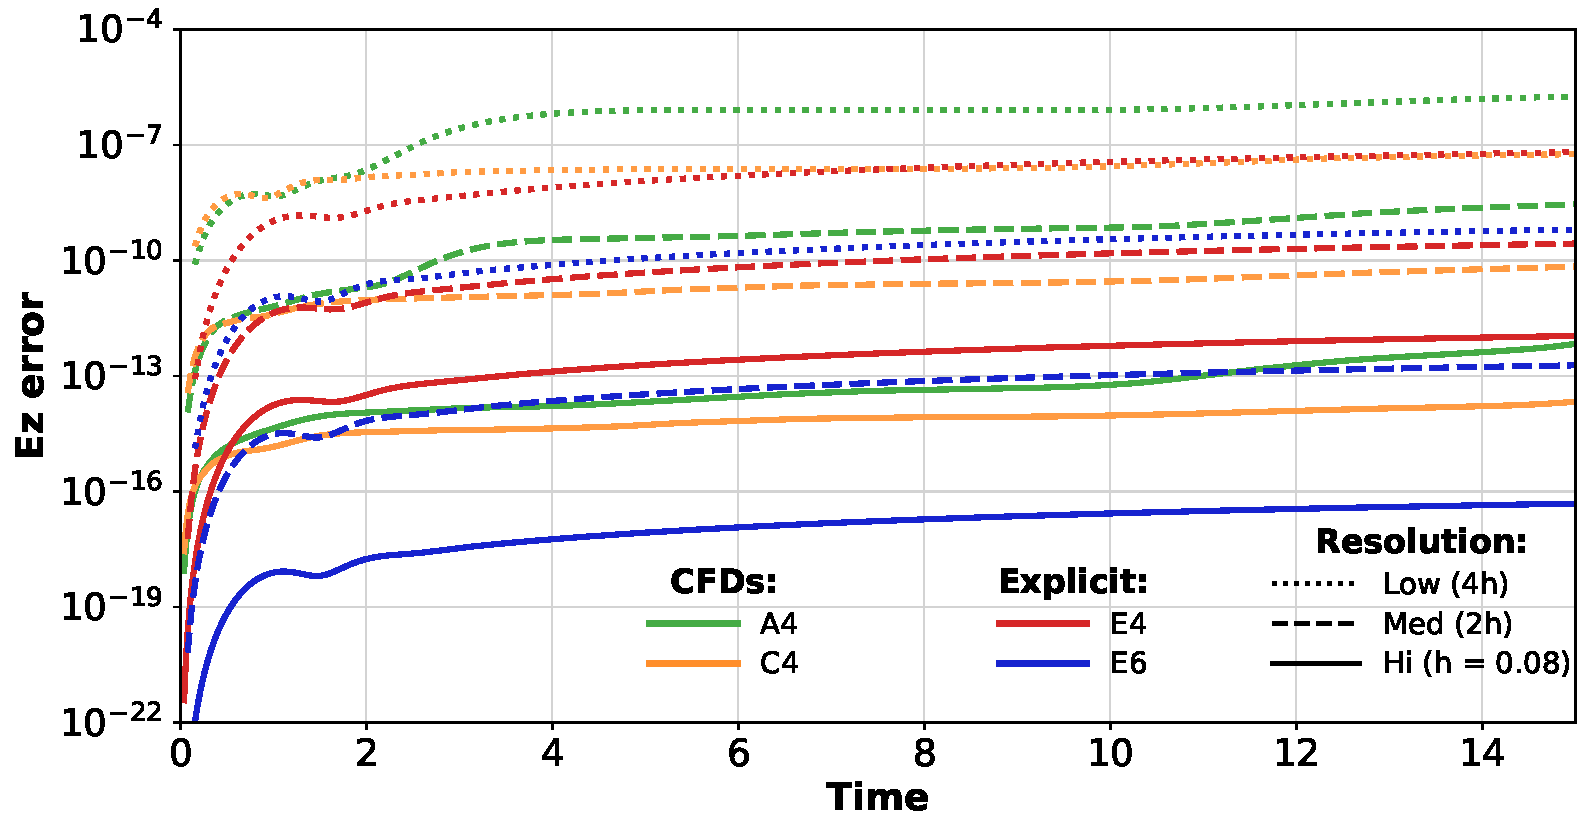
\includegraphics[width=\linewidth]{figures/U_E2_DIFF__ALL_FAMILIES.pdf}
    \vspace{-.75cm}
    \caption{
    Comparison of the errors in the magnetic and electric field components,
    $B_x$ and $E_x$, for different fourth order compact and explicit finite
    difference schemes. We plot the $L_2$ error of the numerical solution
    across the grid relative to the analytic solution. Dotted lines denote
    the low resolution runs, dashed lines denote the medium resolution runs,
    and solid lines denote the high resolution runs. The grid spacing is
    halved between each successive resolution. The fourth order compact
    operators perform comparably to their explicit counterparts at half the
    resolution and achieve error levels comparable to those of the sixth
    order explicit operators. This behavior is observed for both the A4 and
    C4 families of operators tested here.
    }
    \label{fig:maxwell_fourth_order_error}
\end{figure}

\paragraph{Sixth Order Operators}

\begin{figure}[t]
    \centering
    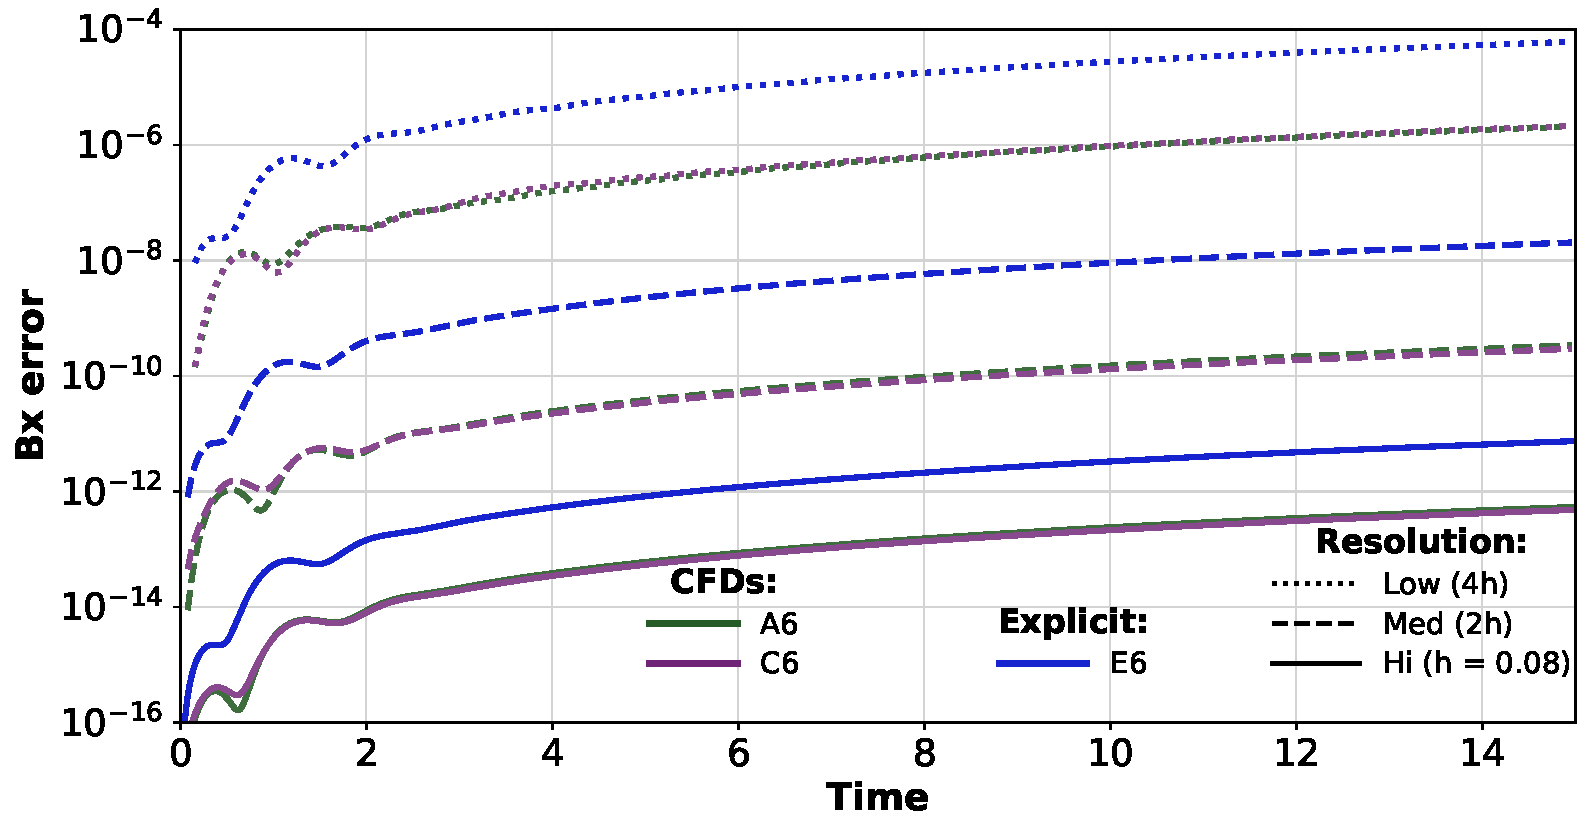
\includegraphics[width=\linewidth]{figures/6th_order_EM4_U_B0_DIFF_ALL_FAMILIES.pdf}
    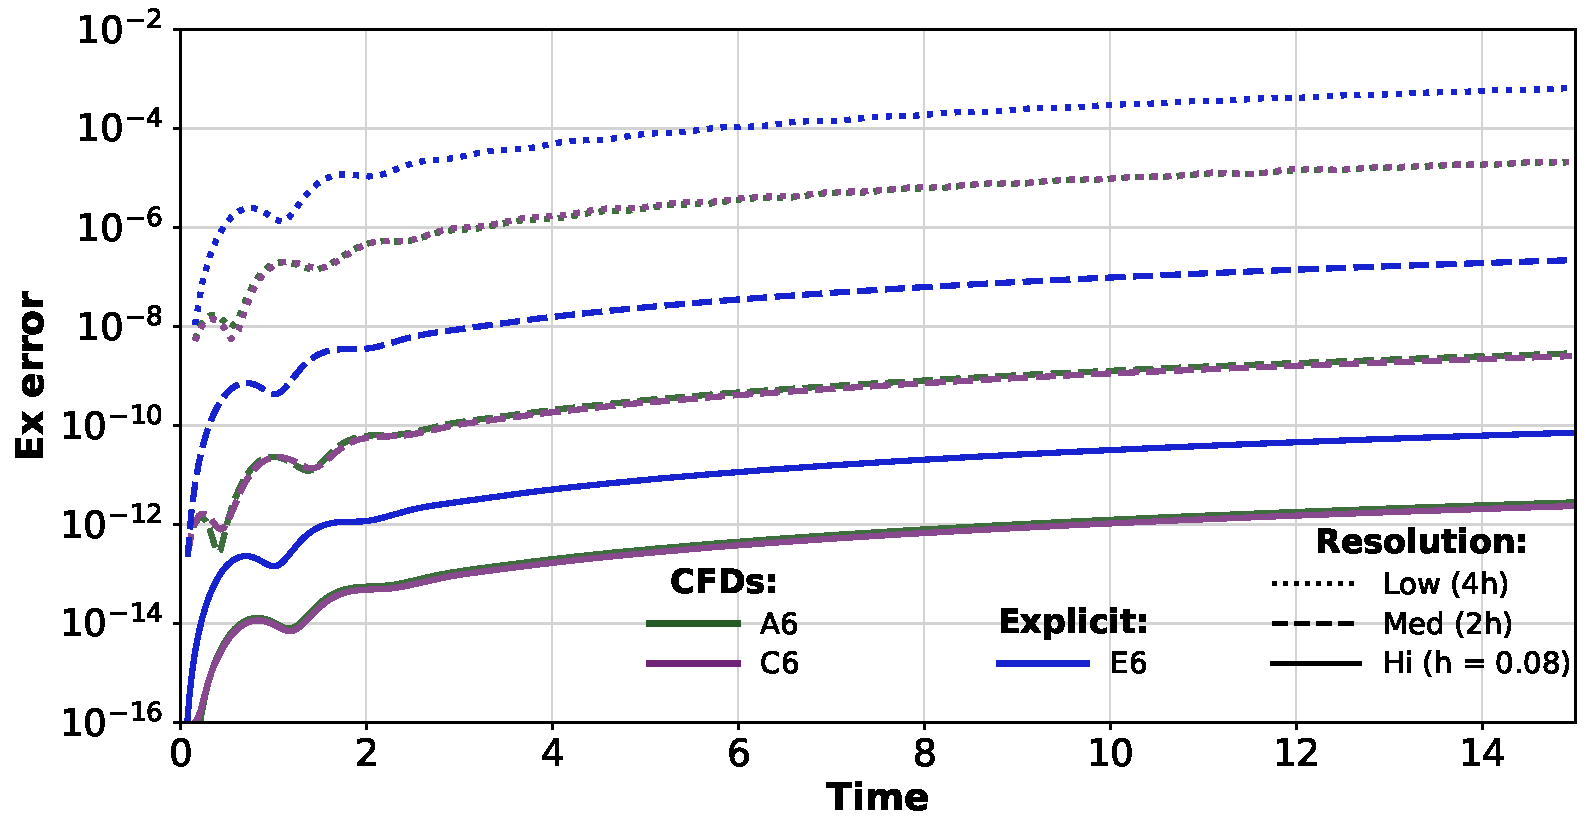
\includegraphics[width=\linewidth]{figures/6th_order_EM4_U_E0_DIFF_ALL_FAMILIES.pdf}
    %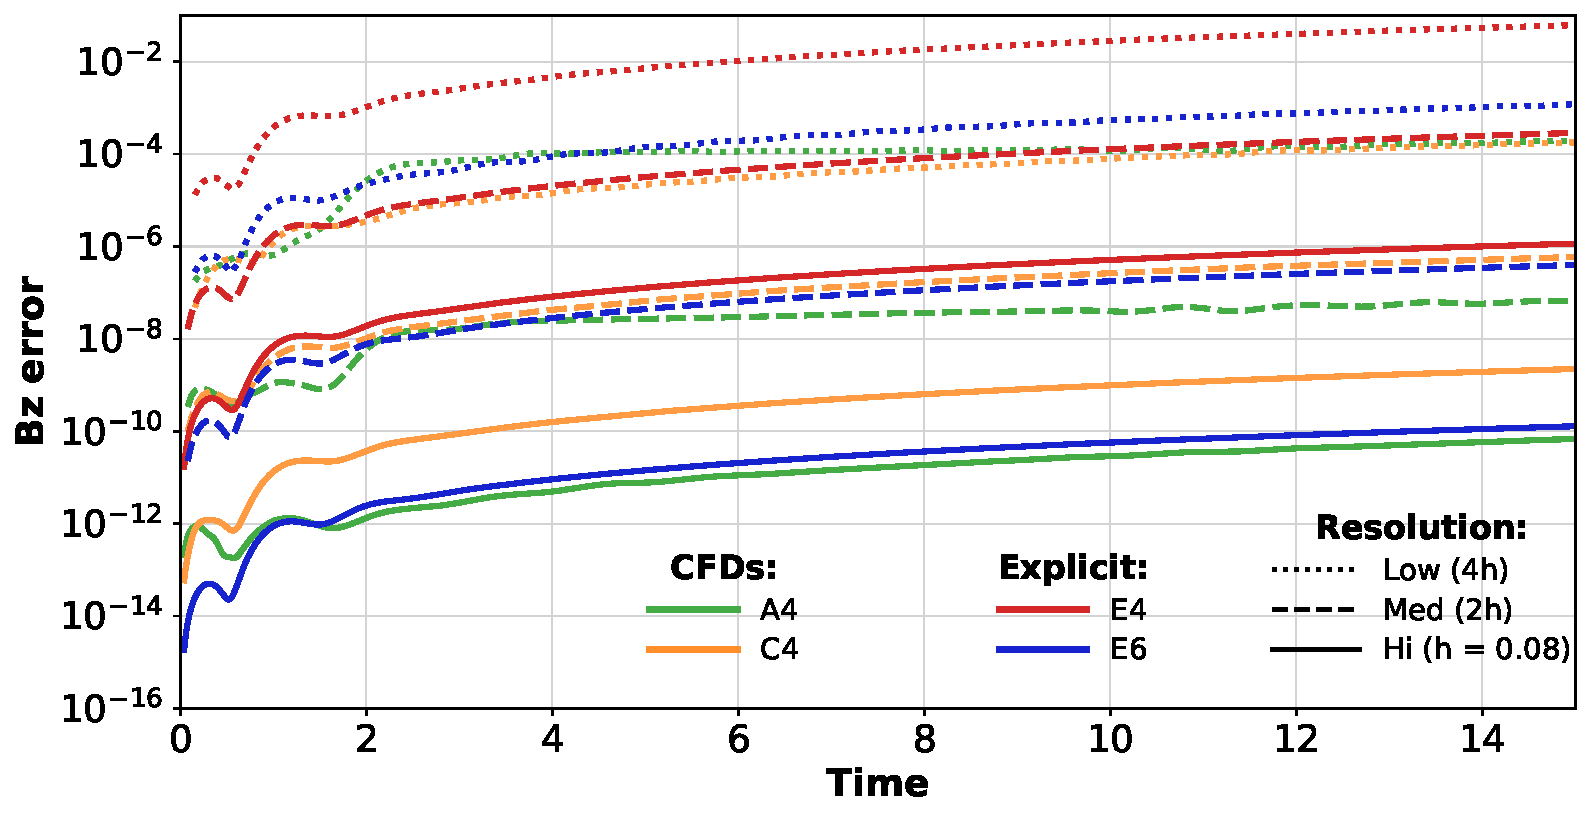
\includegraphics[width=\linewidth]{figures/U_B2_DIFF__ALL_FAMILIES.pdf}
    \vspace{-.75cm}
    \caption{
    Comparison of the errors in the magnetic and electric field components,
    $B_x$ and $E_x$, for different sixth order compact and explicit finite
    difference schemes. We plot the $L_2$ error of the numerical solution
    across the grid relative to the analytic solution. Dotted lines denote
    the low resolution runs, dashed lines denote the medium resolution runs,
    and solid lines denote the high resolution runs. The grid spacing is
    halved between each successive resolution. Although the sixth order
    compact operators do not provide a full factor of two improvement in
    resolution over their explicit counterparts of the same order, they
    still produce more than an order of magnitude improvement in accuracy.
    This behavior is observed for both the A6 and C6 families of operators
    tested here.
    }
    \label{fig:maxwell_sixth_order_error}
\end{figure}
% \begin{figure}\centering
%   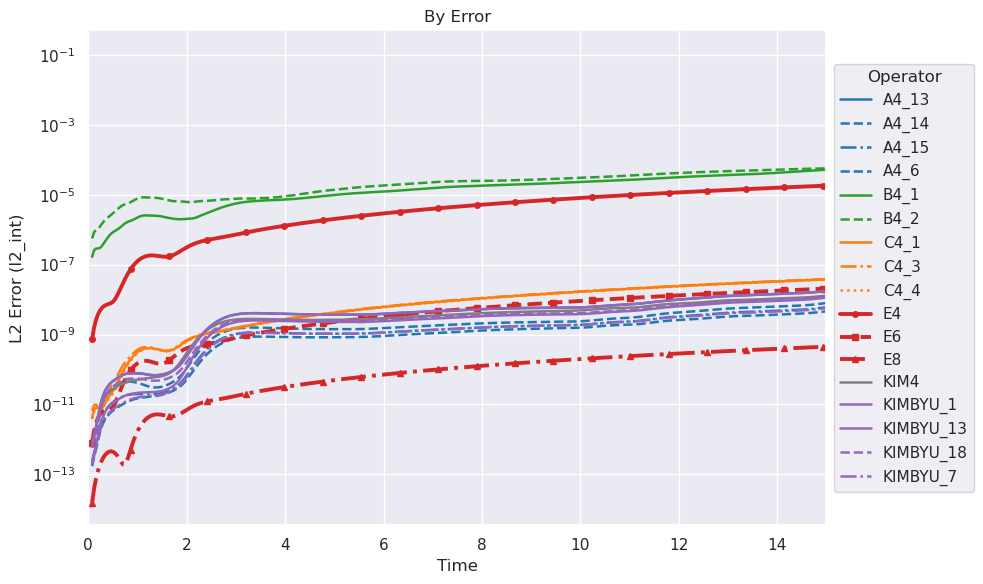
\includegraphics[width=\linewidth]{figures/U_B1_DIFF_error_plots.png}
%   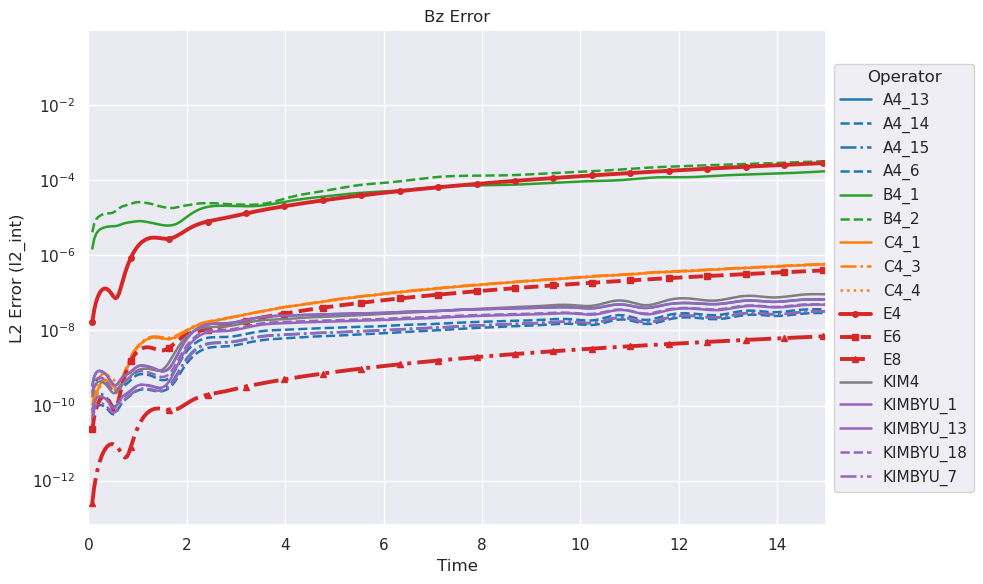
\includegraphics[width=\linewidth]{figures/U_B2_DIFF_error_plots.png}
%   \vspace{-.75cm}
%   \caption{
%     Comparison of error in the magnetic field component, $B_y$, for different CFD and explicit schemes.   component  for $q=4$. 
%     % describe sub-plots
%     We see . 
%   }
%   \label{fig:B_y_Bz_error}
% \end{figure}
% \subsection{Maxwell with second derivatives}
% \ajc{I include these here the 4th order derivatives are fine but I think that the 6th order derivatives really sell us short so I think we may be better sticking to NLSM... but they are here if we change our mind}
% \subsection{4th-order operators}
% \begin{figure}\centering
%   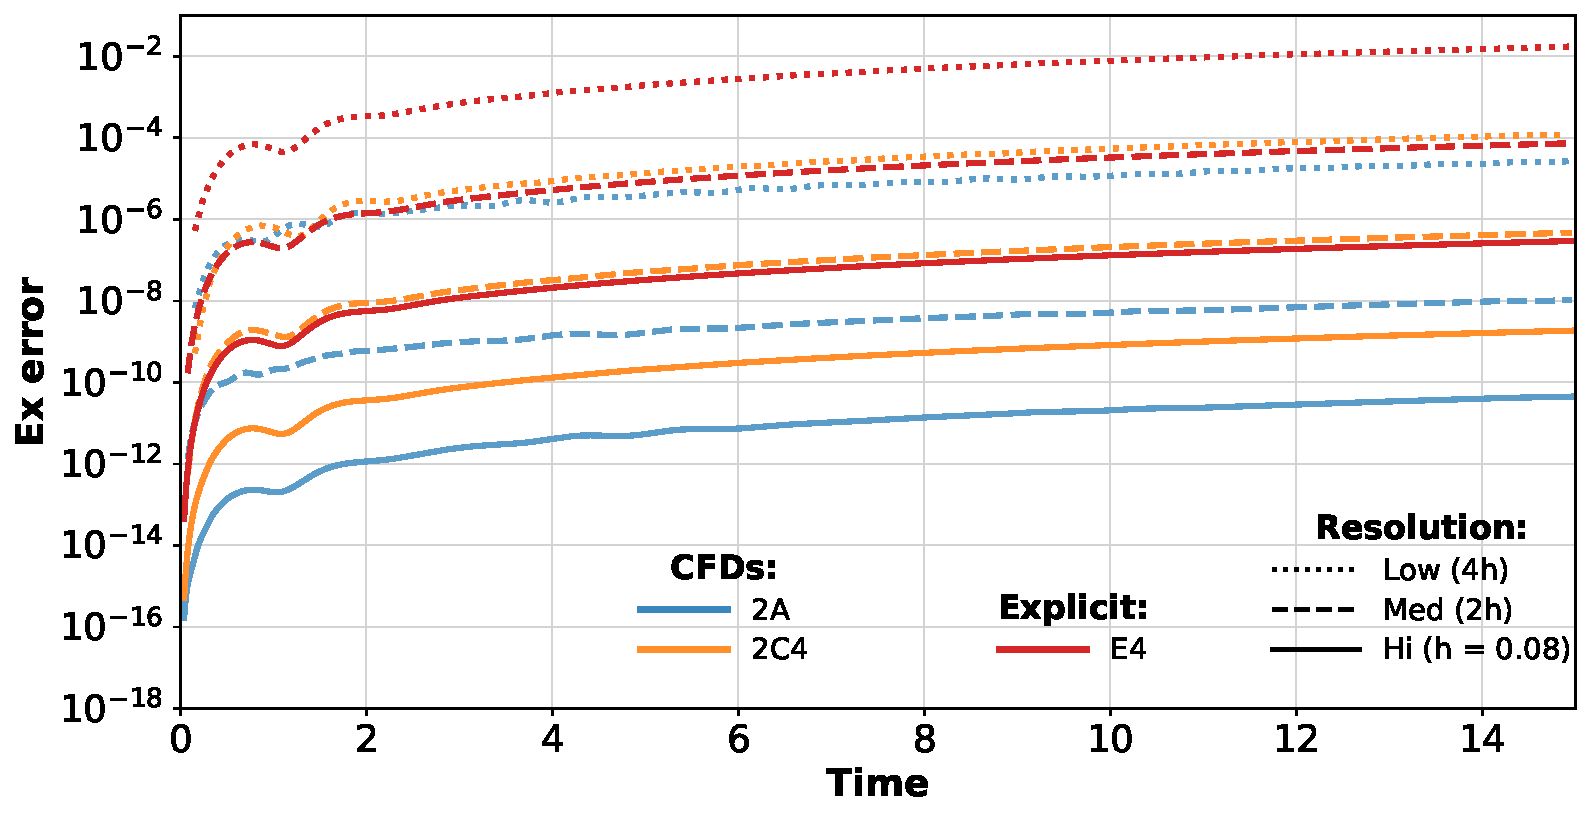
\includegraphics[width=\linewidth]{figures/4th_order_EM2_U_E0_DIFF__ALL_FAMILIES.pdf}
%   %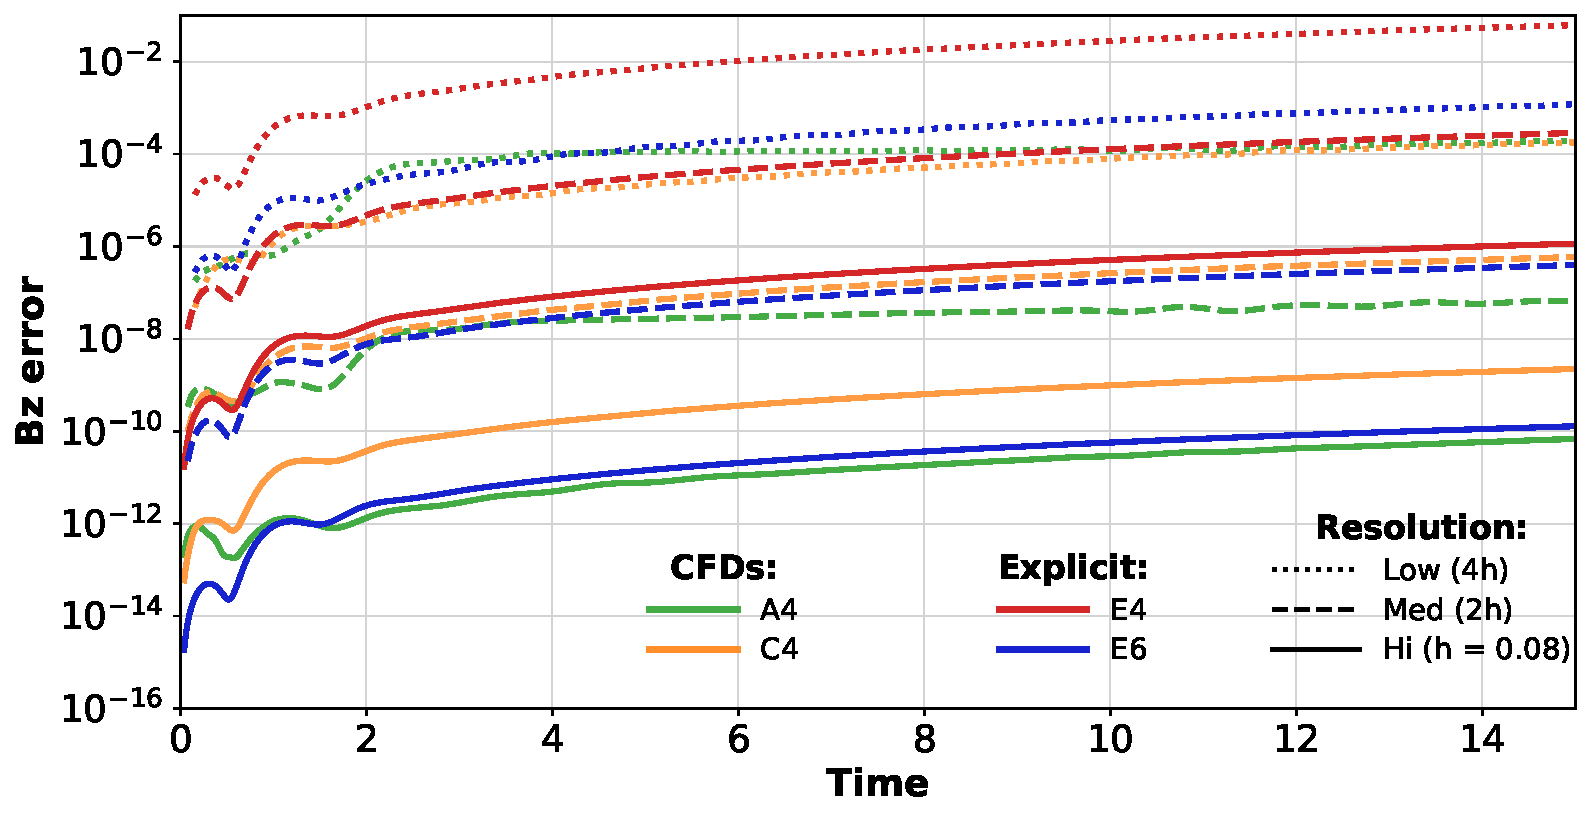
\includegraphics[width=\linewidth]{figures/U_B2_DIFF__ALL_FAMILIES.pdf}
%   \vspace{-.75cm}
%   \caption{
%    Error plot of 4th order derivatives with the second derivative formulation of Maxwell at different resolutions
% }
%   \label{fig:4th_phi_error}
% \end{figure}
% \subsection{Sixth-order operators}
% \begin{figure}\centering
%   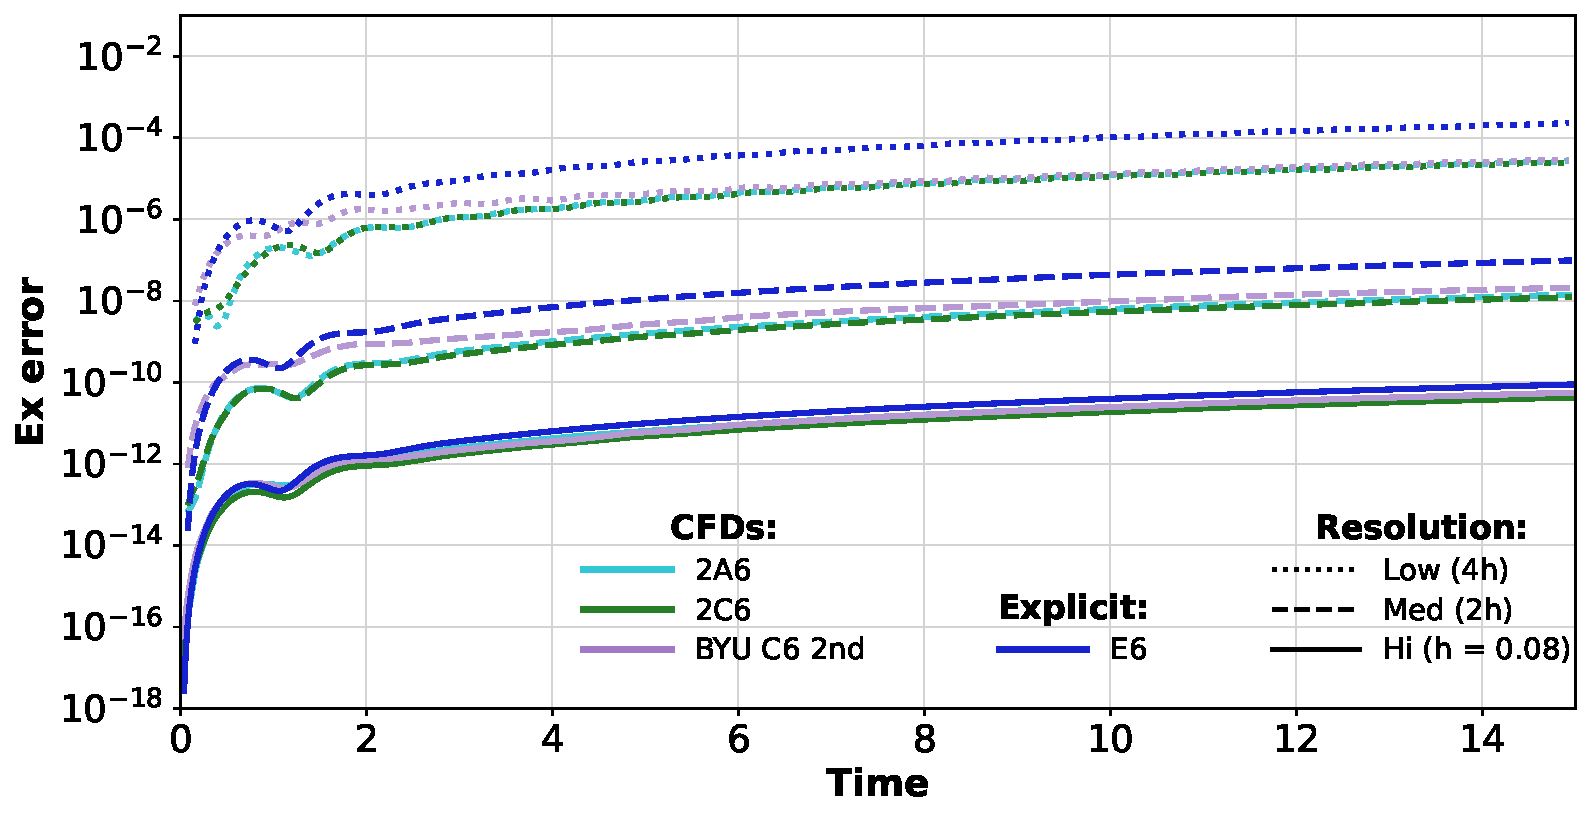
\includegraphics[width=\linewidth]{figures/6th_order_EM2_U_E0_DIFF__ALL_FAMILIES.pdf}
%   %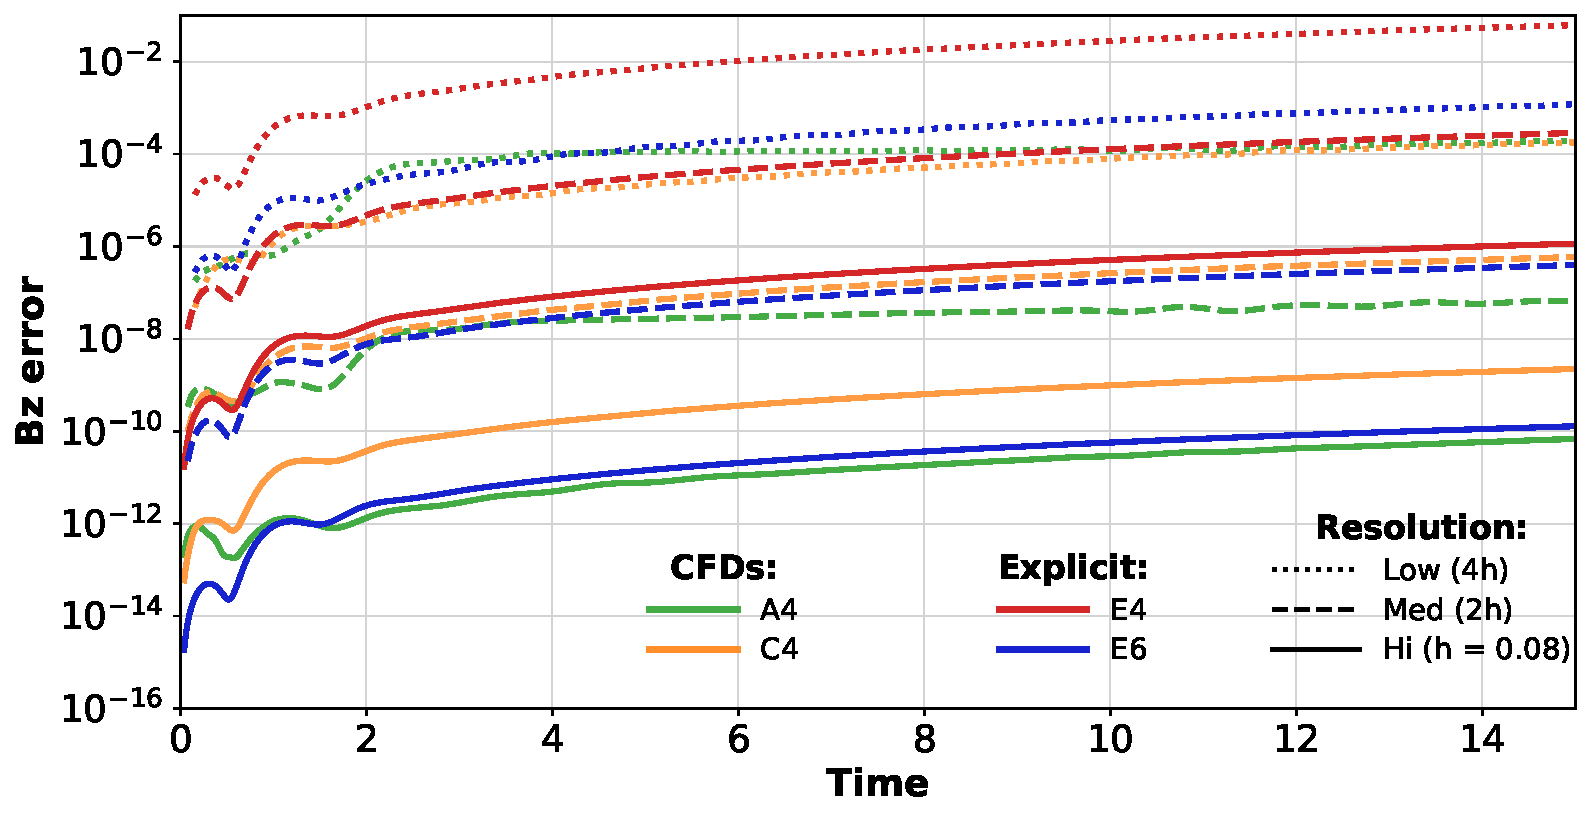
\includegraphics[width=\linewidth]{figures/U_B2_DIFF__ALL_FAMILIES.pdf}
%   \vspace{-.75cm}
%   \caption{
%  Error plot of 6th order derivatives with the second derivative formulation of Maxwell at different resolutions
% }
%   \label{fig:6th_phi_error}
% \end{figure}

\subsection{Nonlinear sigma model}

We next consider the nonlinear sigma model.  This system provides a nonlinear scalar-field test problem and is useful for studying how the different derivative operators behave in the presence of nonlinear source terms.  We evolve the scalar field $\chi$ together with its conjugate momentum $\phi$.

The evolution equations are
\begin{align}
\partial_t \phi
&= \partial_i\partial_i \chi - \frac{\sin(2\chi)}{r^2},
\\
\partial_t \chi
&= \phi .
\end{align}
Here $\partial_i\partial_i$ denotes the flat-space Laplacian.  The term $\sin(2\chi)/r^2$ provides a useful test of the stability and accuracy of the numerical method in nonlinear systems.
In this case we don't have an analytic solution but we do a few convergence tests shown in figure blah. This gives us the change to confirm that our operators work even in a nonlinear system and converge at the expected order.  We use initial data given as follows:
 The scalar field is initialized as
\begin{equation}
\chi(x,y,z)
=
A
\exp\left[
-\frac{(\tilde r-R)^2}{\delta^2}
\right],
\end{equation}
where
\begin{equation}
\tilde r
=
\sqrt{
\epsilon_x(x-x_c)^2
+
\epsilon_y(y-y_c)^2
+
\epsilon_z(z-z_c)^2
}.
\end{equation}
The conjugate momentum is initially set to
\begin{equation}
\phi(x,y,z)=0.
\end{equation}

For the simulations considered here, we choose
\begin{equation}
A=1,\qquad
\delta=3,\qquad
x_c=y_c=z_c=0,
\end{equation}
together with
\begin{equation}
\epsilon_x=\epsilon_y=\epsilon_z=1,
\qquad
R=0.
\end{equation}
Thus, the initial scalar profile is a spherically symmetric Gaussian centered
at the origin. The wave speeds in all three spatial directions are set to
unity.
%\ajc{I have added in convergence plots, I will probably update these but the story shouldn't change too much}

\paragraph{Fourth Order Operators}

\begin{figure}[t]
    \centering
    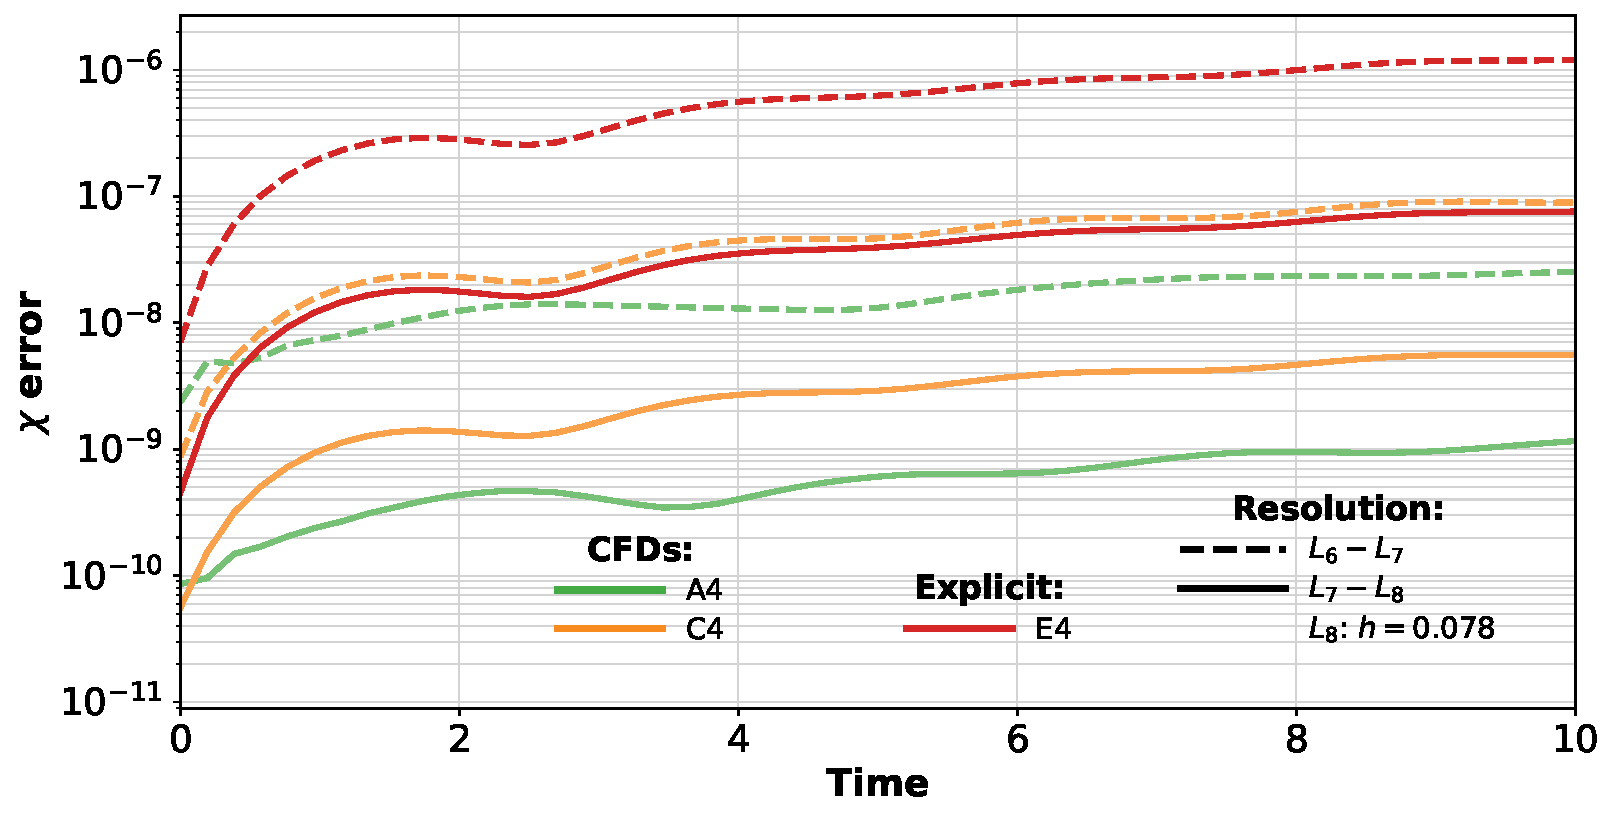
\includegraphics[width=\linewidth]{figures/4th_order_U_CHI_ALL_FAMILIES.pdf}
    %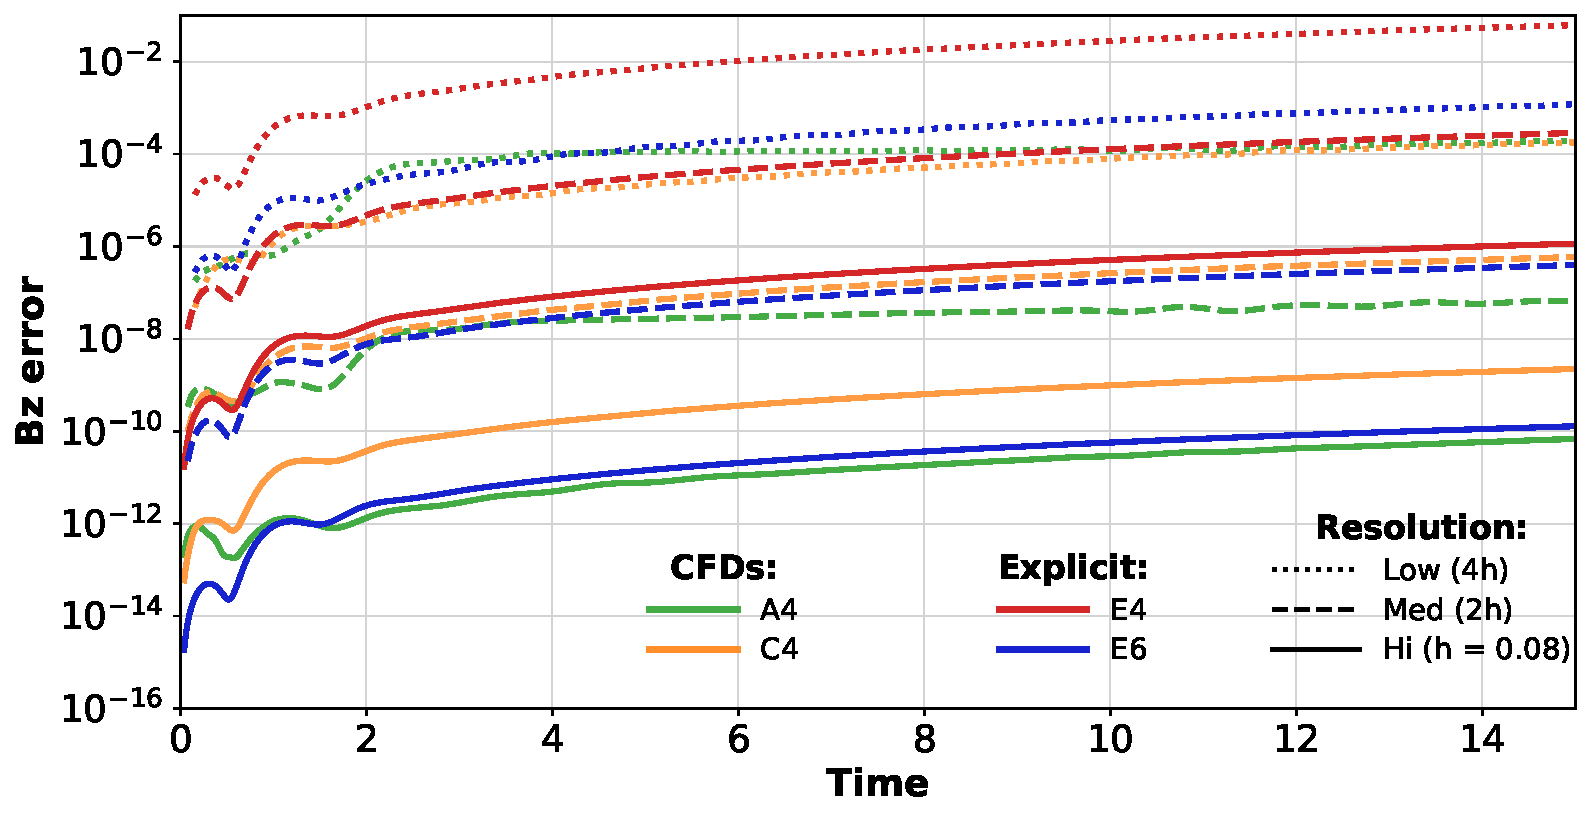
\includegraphics[width=\linewidth]{figures/U_B2_DIFF__ALL_FAMILIES.pdf}
    \vspace{-.75cm}
    \caption{
    Convergence of the nonlinear sigma model field $\phi$ for the fourth
    order compact and explicit finite difference schemes. The plotted
    quantity is the difference between successive resolutions. Dotted lines
    denote the low and medium resolution comparison, dashed lines denote the
    medium and high resolution comparison, and solid lines denote the highest
    resolution run. The grid spacing is halved between each successive
    resolution. The compact operators remain stable in the nonlinear system. Notice that again in this nonlinear system the 4th order A4 and C4 operators perform the same as the Explicit 4th order at half od the resolution. 
    }
    \label{fig:nlsm_fourth_order_error}
\end{figure}

\paragraph{Sixth Order Operators}

\begin{figure}[t]
    \centering
    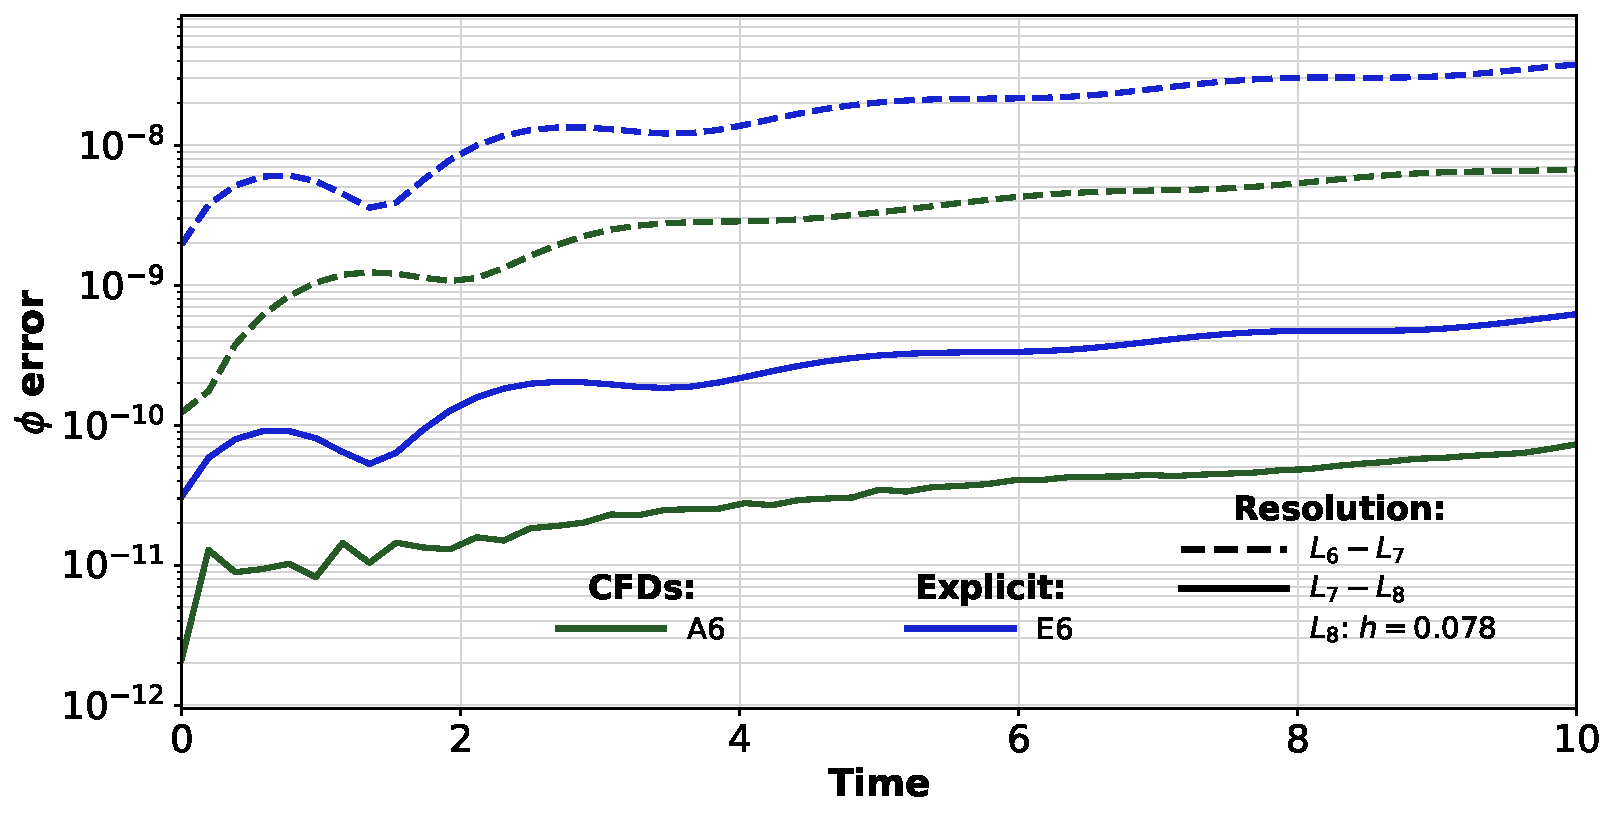
\includegraphics[width=\linewidth]{figures/6th_order_U_PHI_ALL_FAMILIES.pdf}
    %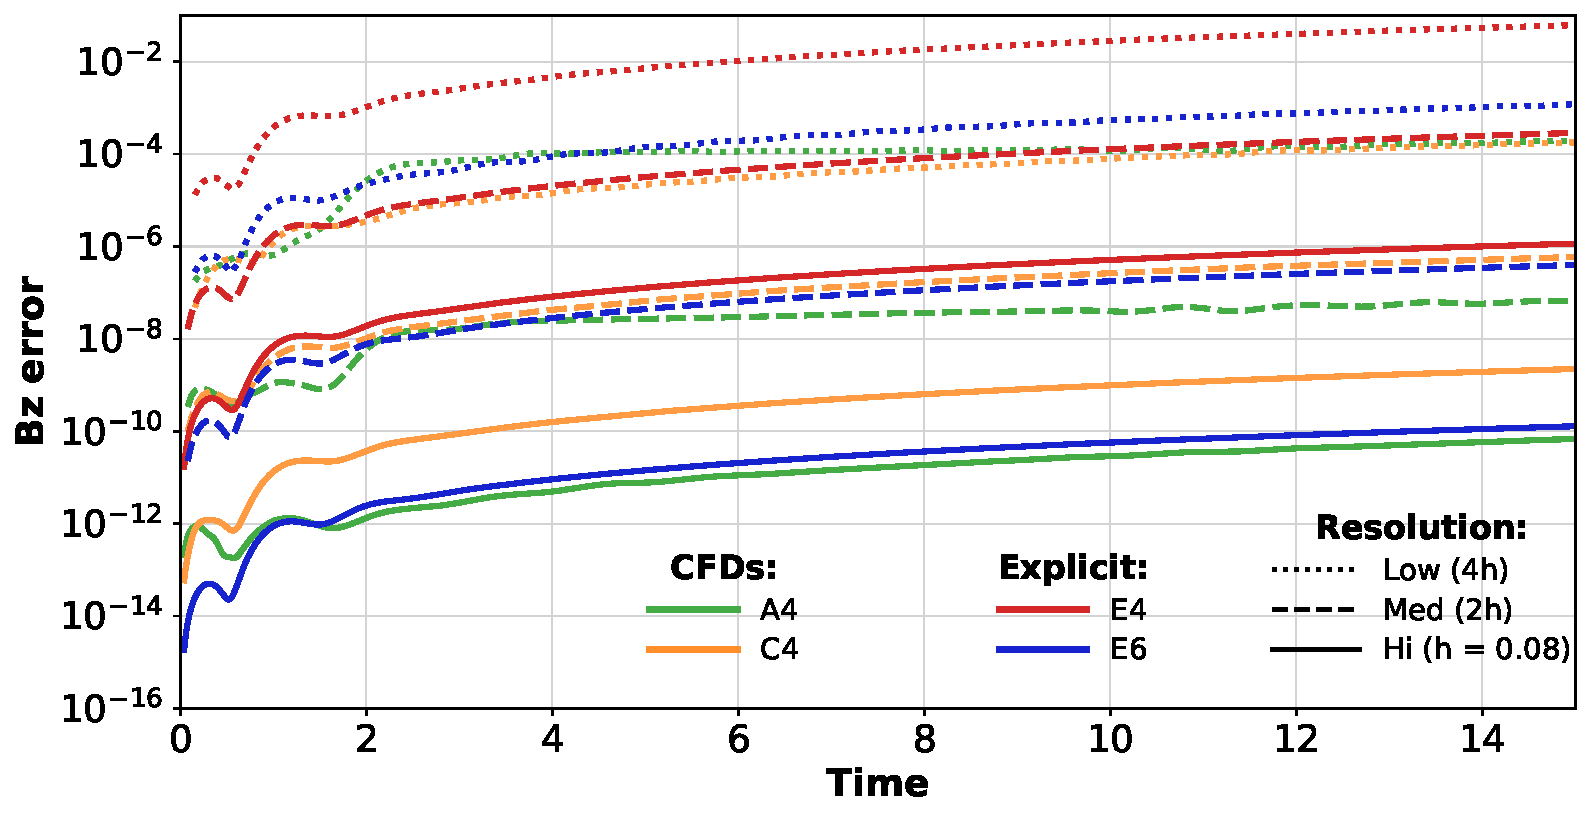
\includegraphics[width=\linewidth]{figures/U_B2_DIFF__ALL_FAMILIES.pdf}
    \vspace{-.75cm}
    \caption{
    Convergence of the nonlinear sigma model field $\phi$ for the sixth
    order compact and explicit finite difference schemes. The plotted
    quantity is the difference between successive resolutions. Dotted lines
    denote the low and medium resolution comparison, dashed lines denote the
    medium and high resolution comparison, and solid lines denote the highest
    resolution run. The grid spacing is halved between each successive
    resolution. We do not seem to get the full order of resolution improvement that we got with the 4th order operators but we do seem to get close to an order of magnitude improvement..
    }
    \label{fig:nlsm_sixth_order_error}
\end{figure}
\subsection{Gravitational Waves}

We also test the derivative operators by evolving Teukolsky-wave initial data with the full BSSN equations.  The BSSN formulation is described in detail elsewhere, for example in Ref.~\cite{Baumgarte2010}.  These data describe a linearized gravitational-wave perturbation of the metric and provide a useful test problem for wave propagation in a numerical relativity setting.

For the results shown here, we perform direct convergence tests rather than
comparing against an analytic solution. The computational domain extends over
$x,y,z\in[-40,40]$, and the initial perturbation is centered at radius
$r_0=20.0$. We use outgoing, even-parity Teukolsky-wave initial data in the
quadrupolar mode $(\ell,m)=(2,0)$ with amplitude $\mathcal{A}=10^{-2}$. The
radial profile is a compactly supported $C^k$ polynomial with $k=6$ and
half-width $w=2.0$. A representative visualization of the resulting evolution
is shown in Fig.~\ref{fig:bssn_gt00_panel}.

\begin{figure}[t]
    \centering
    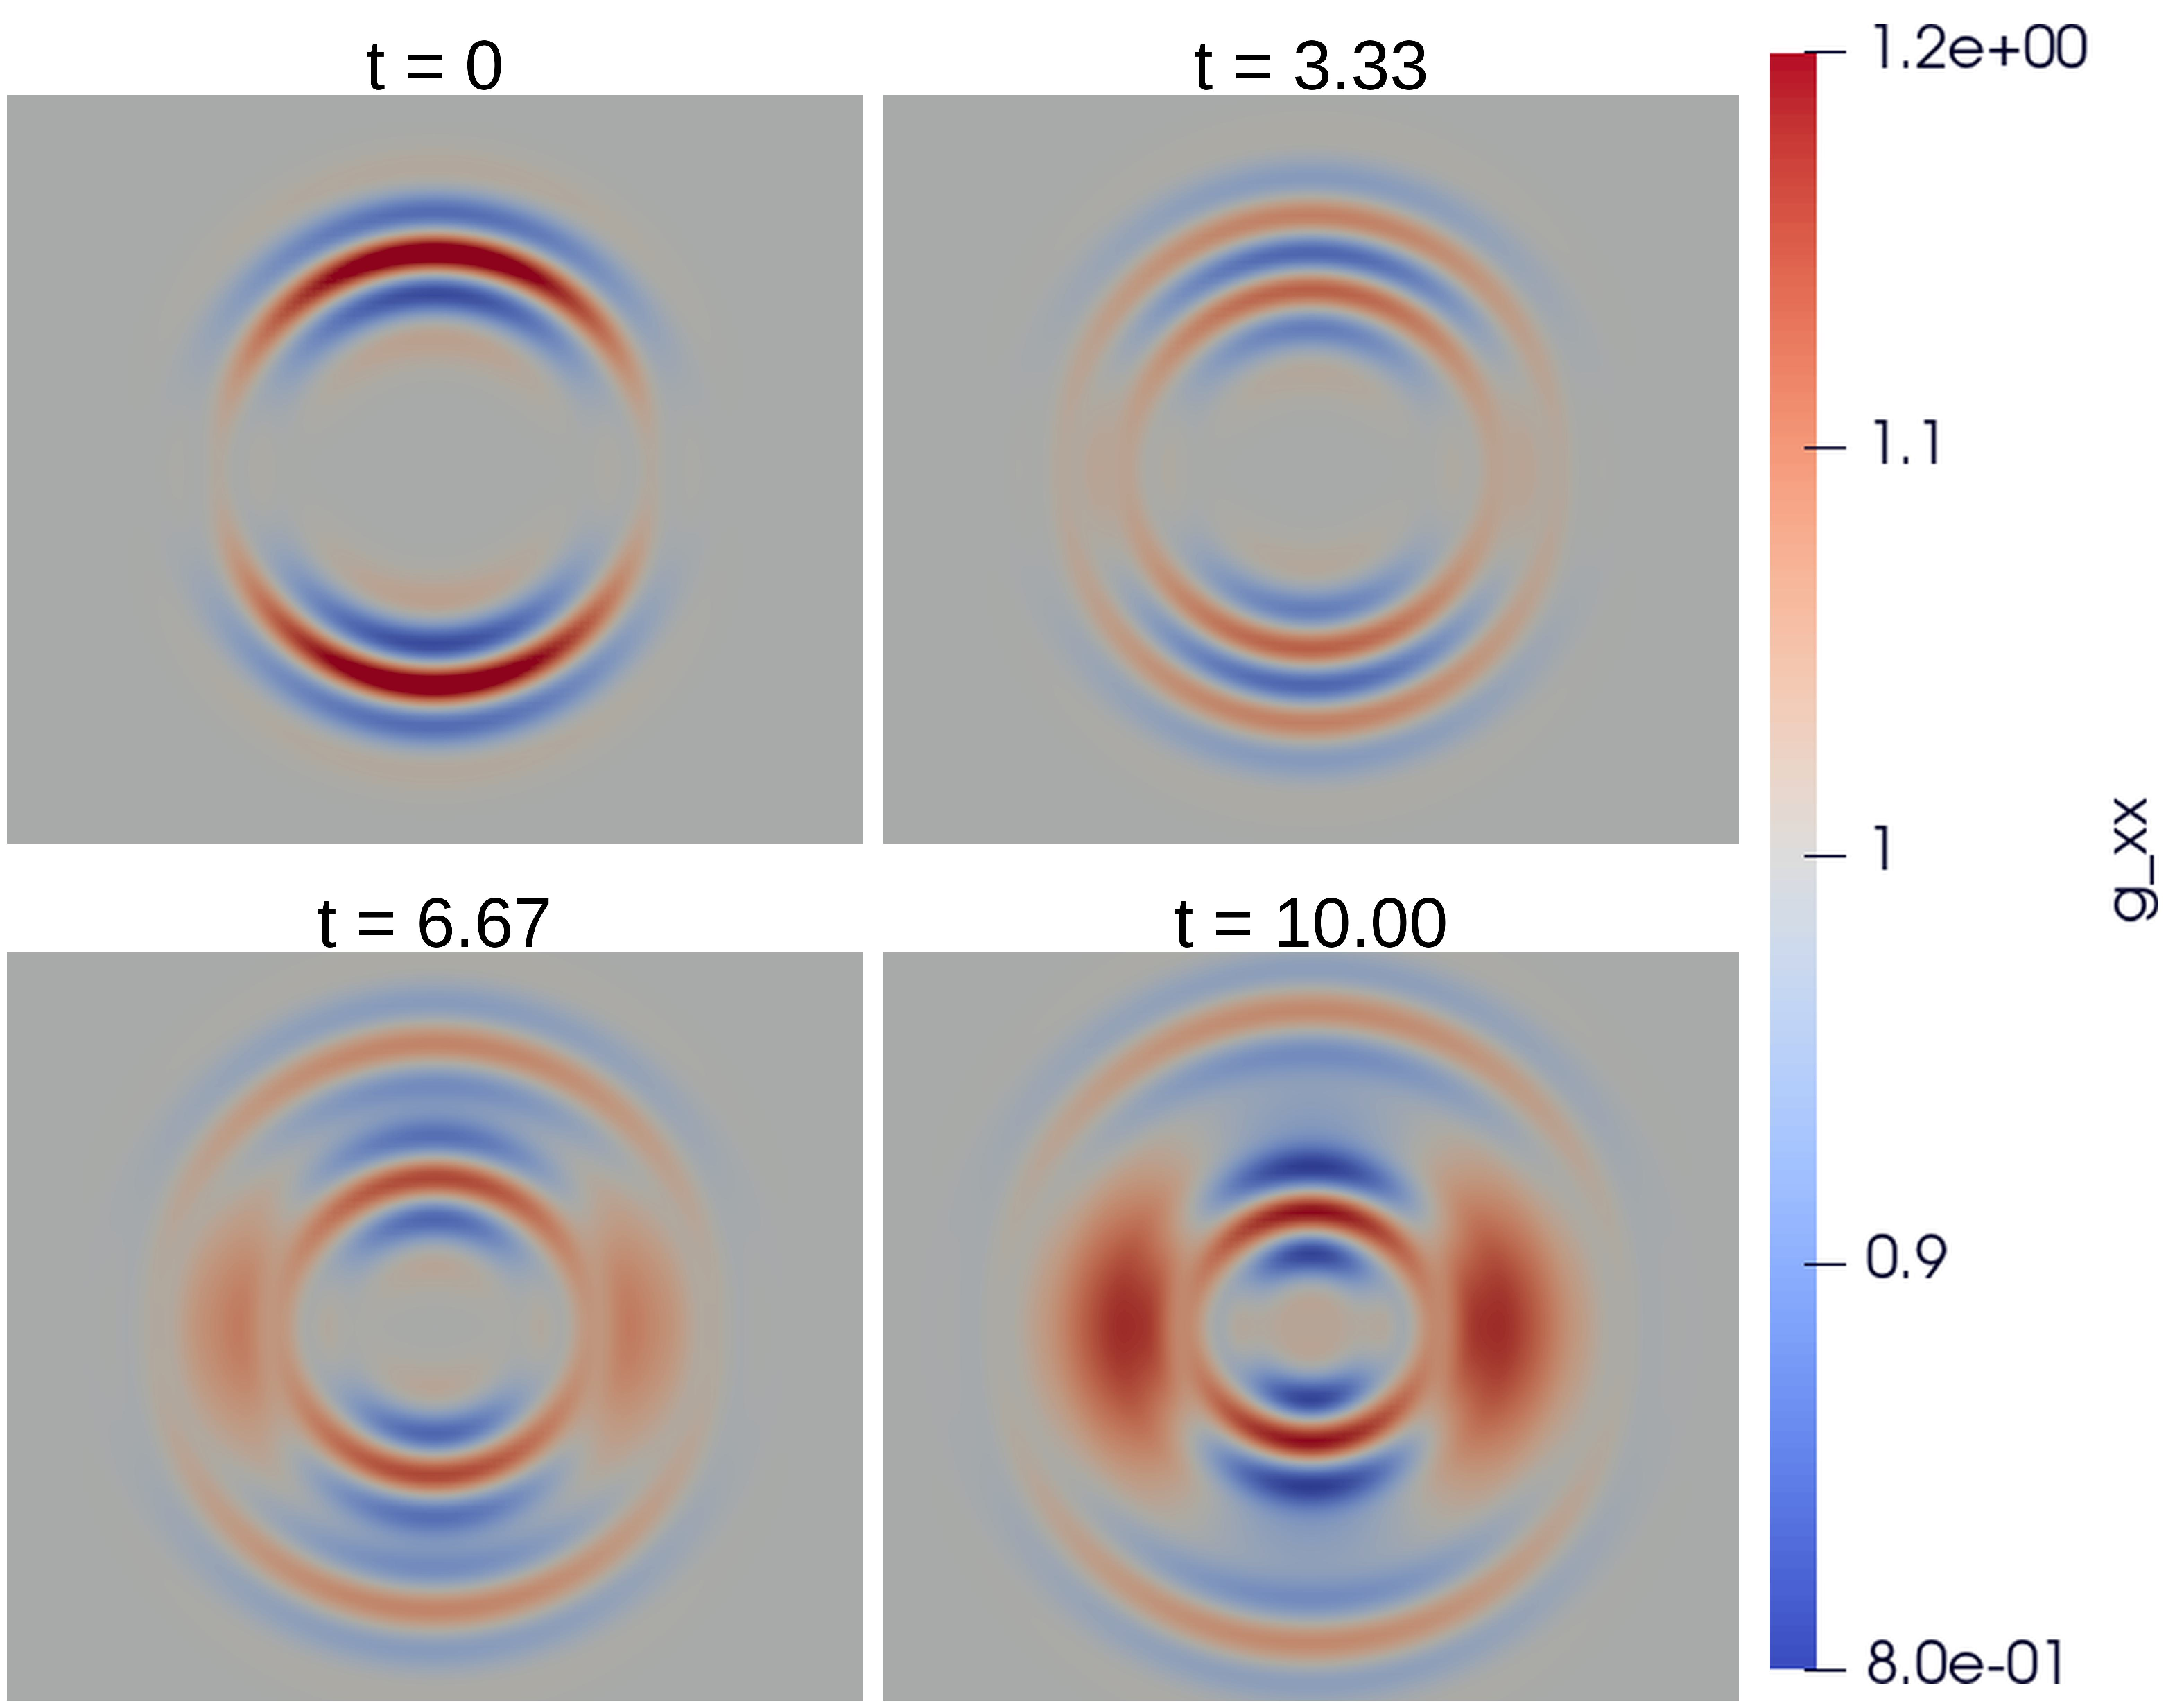
\includegraphics[width=\columnwidth]{figures/GT00_panel.pdf}
    \caption{
    Evolution of the metric component $g_{xx}$ for the Teukolsky-wave test problem.
    The panels show snapshots at $t=0$, $t=3.33$, $t=6.67$, and $t=10.00$.
    The shared color scale on the right applies to all four panels.
    }
    \label{fig:bssn_gt00_panel}
\end{figure}

\paragraph{Fourth Order Operators}

\begin{figure}[t]
    \centering
    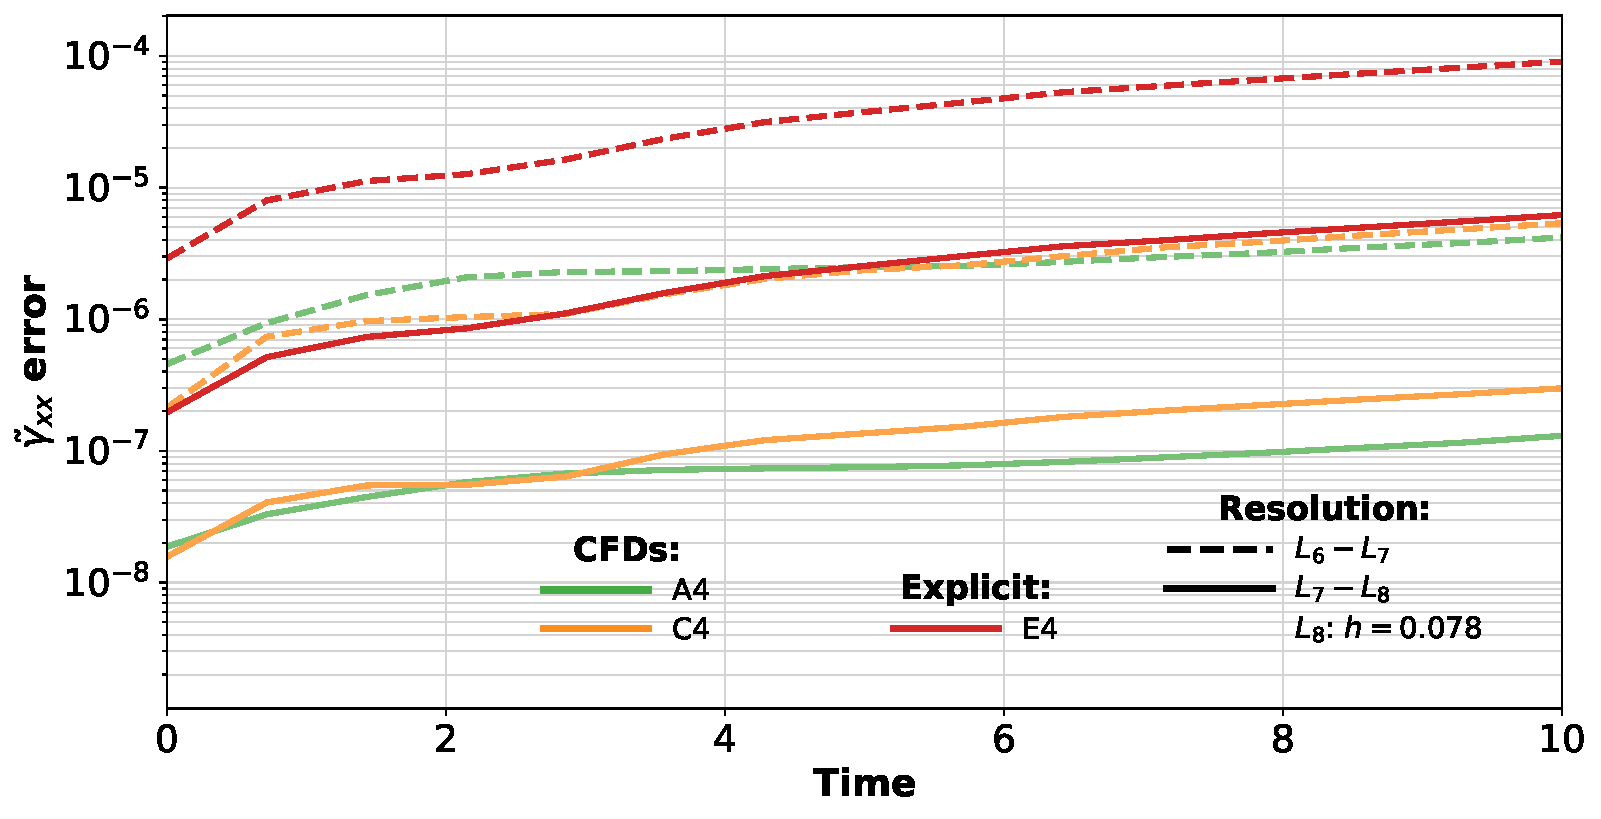
\includegraphics[width=\linewidth]{figures/4th_order_U_SYMGT0_ALL_FAMILIES.pdf}
    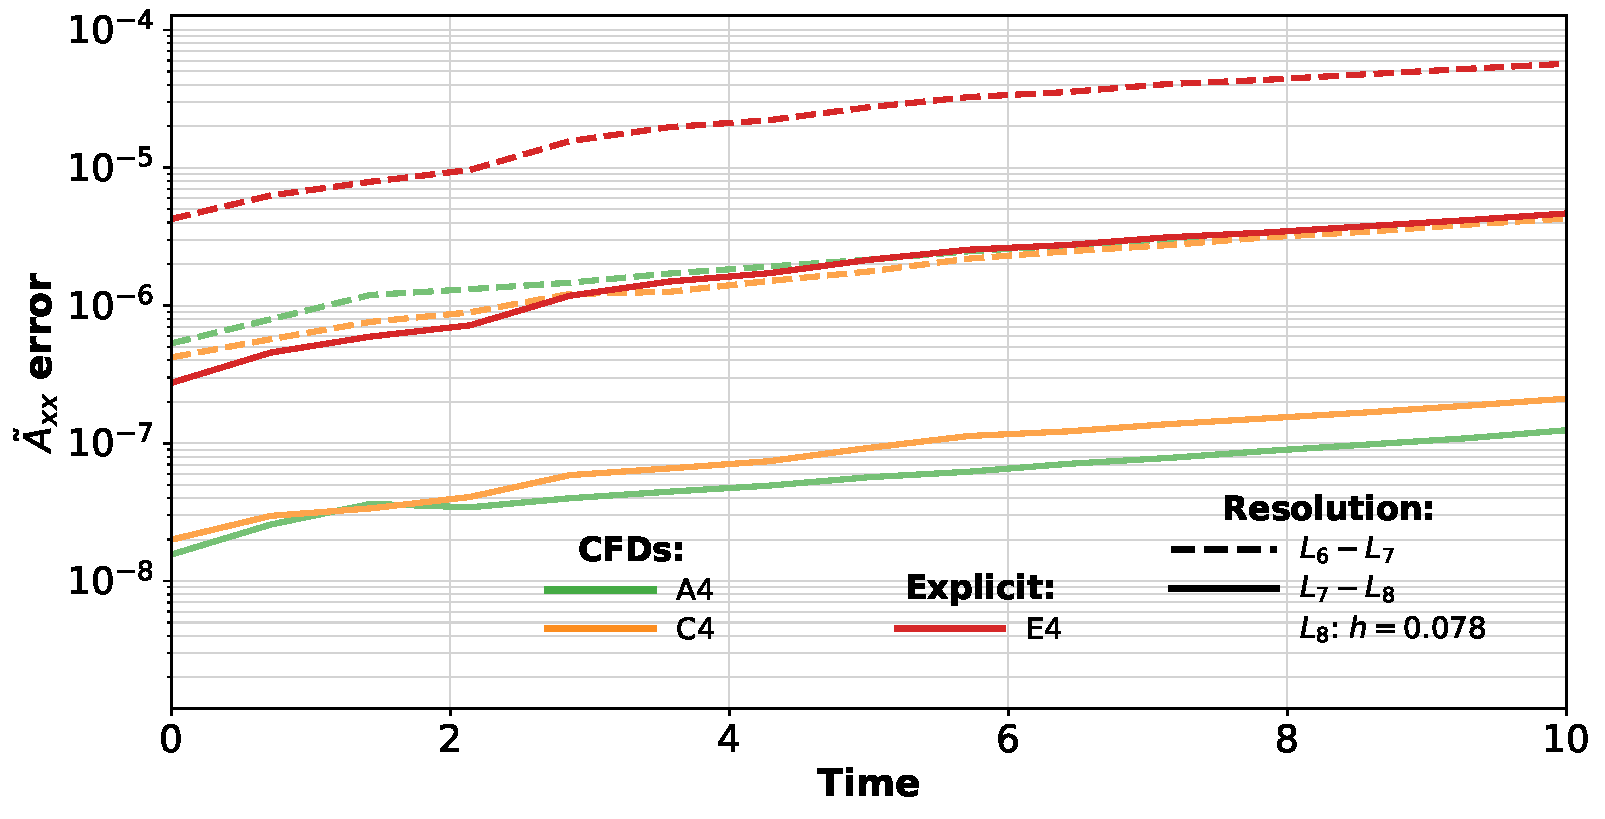
\includegraphics[width=\linewidth]{figures/4th_order_U_SYMAT0_ALL_FAMILIES.pdf}
    \vspace{-.75cm}
    \caption{
    Convergence of the metric component $g_{xx}$ and the conformal extrinsic
    curvature component $\tilde{A}_{xx}$ for the fourth order compact and
    explicit finite difference schemes. The plotted quantities are the
    differences between successive resolutions. Dotted lines denote the low
    and medium resolution comparison, dashed lines denote the medium and high
    resolution comparison, and solid lines denote the highest resolution run.
    The grid spacing is halved between each successive resolution. The compact
    operators remain stable during the Teukolsky wave evolution. Notice that,
    as in the nonlinear sigma model, the fourth order A4 and C4 operators
    perform comparably to the explicit fourth order operator at half the
    resolution.
    }
    \label{fig:teukolsky_fourth_order_error}
\end{figure}

\paragraph{Sixth Order Operators}

\begin{figure}[t]
    \centering
    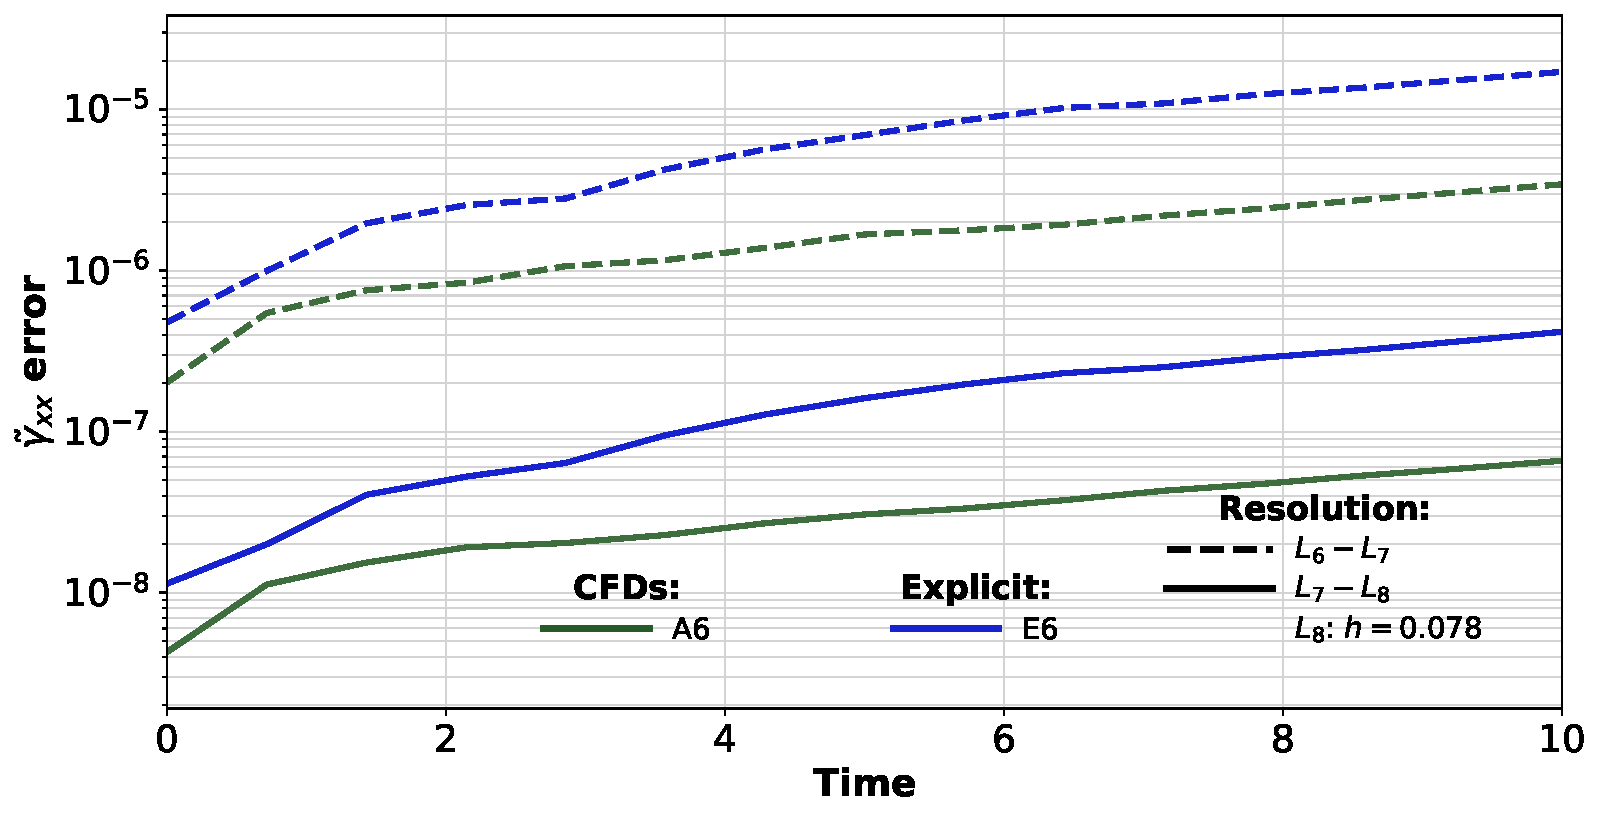
\includegraphics[width=\linewidth]{figures/6th_order_U_SYMGT0_ALL_FAMILIES.pdf}
    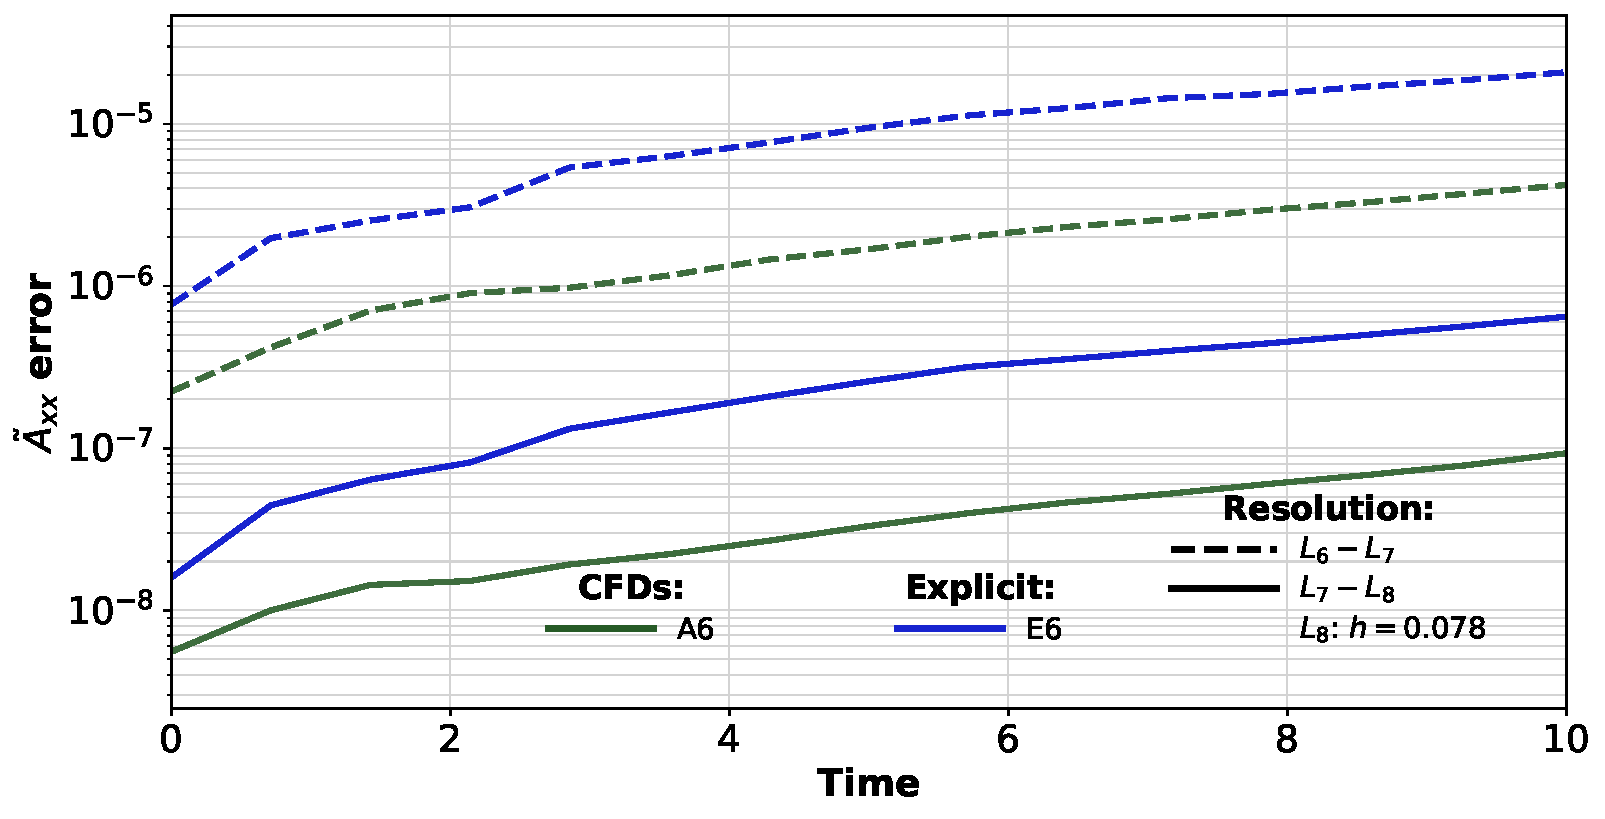
\includegraphics[width=\linewidth]{figures/6th_order_U_SYMAT0_ALL_FAMILIES.pdf}
    \vspace{-.75cm}
    \caption{
    Convergence of the metric component $g_{xx}$ and the conformal extrinsic
    curvature component $\tilde{A}_{xx}$ for the sixth order compact and
    explicit finite difference schemes. The plotted quantities are the
    differences between successive resolutions. Dotted lines denote the low
    and medium resolution comparison, dashed lines denote the medium and high
    resolution comparison, and solid lines denote the highest resolution run.
    The grid spacing is halved between each successive resolution. As in the
    nonlinear sigma model, the sixth order compact operators do not achieve
    the full resolution improvement seen for the fourth order operators, but
    they still provide close to an order of magnitude improvement in accuracy.
    }
    \label{fig:teukolsky_sixth_order_error}
\end{figure}
\section{Conclusion}
\label{sec:conclusion}

The compact operators consistently produced smaller errors than explicit
finite difference operators of the same nominal order. In the fourth order
tests, the compact operators frequently achieved errors comparable to those
of the explicit operators evaluated at twice the resolution. They also
produced error levels comparable to sixth order explicit operators in several
of the Maxwell tests. The sixth order compact operators did not always provide
a full factor of two improvement in effective resolution, but they commonly
reduced the error by approximately an order of magnitude relative to their
explicit counterparts.

These improvements were observed in the Maxwell system, the nonlinear sigma
model, and evolutions of Teukolsky gravitational wave initial data using the
BSSN equations. The results therefore indicate that the benefits of the
compact operators are not limited to simple linear systems. In particular,
the operators remained stable and retained their accuracy improvements in
nonlinear and numerical relativity test problems.

Compact finite differences require the solution of an implicit matrix system,
but the fixed size leaf nodes used by \dendrogr\ allow these systems to be
solved efficiently using vectorized linear algebra routines. The additional
cost of the compact derivative calculation may therefore be offset by the
ability to obtain a given error at a lower grid resolution. For
three dimensional time dependent simulations, even a modest reduction in the
required resolution could lead to substantial savings in computational cost.

The next step is to apply these operators to fully nonlinear binary black hole
simulations on adaptive meshes. These tests will determine how the operators
behave near punctures, across refinement boundaries, and during long
inspiral evolutions. They will also allow direct comparisons of waveform
accuracy and computational cost between compact and explicit finite
difference methods. The results presented here suggest that compact finite
differences provide a promising route toward more accurate gravitational
waveforms without requiring a corresponding increase in computational
expense. We already have some tentative results showing that CFDs perform well
in full binary black hole systems, which we present in
Appendix~\ref{sec:black_hole_merger_tests}. In those cases, we show that the
fourth order compact operators perform better than their explicit counterparts.